\documentclass[12pt]{article}
\usepackage{amsmath}
\usepackage{graphicx}
\usepackage{booktabs}
\usepackage{geometry}
\usepackage{multirow}
\usepackage{tabularx}
\usepackage{ulem}
\usepackage{hyperref}
\usepackage{siunitx}
\usepackage{subcaption}
\usepackage{amsmath}
\usepackage{longtable}
\usepackage{changepage} % For adjustwidth environment
\documentclass{article}
\usepackage{amssymb} % For checkmark symbols (\checkmark)
\usepackage{booktabs} % For professional tables
\usepackage{array}

\usepackage{xcolor} % For colored code
\usepackage{listings}
\lstset{
  basicstyle=\ttfamily\small,
  keywordstyle=\color{blue}\bfseries,
  commentstyle=\color{green!70!black},
  stringstyle=\color{orange},
  showstringspaces=false,
  numbers=left,
  numberstyle=\tiny\color{gray},
  frame=single,
  breaklines=true
}


\usepackage{graphicx} % Required for inserting images
\usepackage{graphicx} % Required for inserting images
\usepackage{float}
\usepackage{array}

\usepackage[a4paper, margin=1in]{geometry}

\geometry{a4paper, margin=1in}
\title{Faculty of Engineering -- Cairo University \\ 
Electronics and Electrical Communication Engineering Department \\
Fourth Year -- Mainstream \\ 
Neural Networks: ELC4028 \\ 
Assignment 1: Classical ML Methods}
\author{Submitted to Dr. Mohsen}
\date{}

\begin{document}
\maketitle

\begin{table}[h]
    \centering
    \begin{tabular}{ccc}
        \toprule
        \textbf{Members} & \textbf{Section} & \textbf{ID} \\
        \midrule
        Reem Mahmoud Mohamed & 2 & 9210430 \\
        Salma Mohamed Hamed & 2 & 9210480 \\
        Youssef Hesham Abd-El-Fatah & 4 & 9211451 \\
        \bottomrule
    \end{tabular}
    \caption{Team Members}
    \label{tab:team}
\end{table}


\newpage

\section*{Part 1: Regressing Problems}
\subsection*{Problem 1}
\begin{table}[h!]
    \centering
    \caption{Regression Calculations}
    \begin{tabular}{ccccc}
        \toprule
        \(X_i\) & \(Y_i\) & \(X_i^2\) & \(Y_i^2\) & \(X_i Y_i\) \\
        \midrule
        1987 & 13300 & 3,948,169 & 176,890,000 & 26,427,100 \\
        1988 & 12400 & 3,952,144 & 153,760,000 & 24,651,200 \\
        1989 & 10900 & 3,956,121 & 118,810,000 & 21,680,100 \\
        1990 & 10100 & 3,960,100 & 102,010,000 & 20,099,000 \\
        1991 & 10150 & 3,964,081 & 103,022,500 & 20,208,650 \\
        1992 & 10000 & 3,968,064 & 100,000,000 & 19,920,000 \\
        1993 & 800 & 3,972,049 & 640,000 & 1,594,400 \\
        1994 & 9000 & 3,976,036 & 81,000,000 & 17,946,000 \\
        1995 & 8750 & 3,980,025 & 76,562,500 & 17,456,250 \\
        1996 & 8100 & 3,984,016 & 65,610,000 & 16,167,600 \\
        \midrule
        \(\sum = 19915\) & \(\sum = 93500\) & \(\sum = 39,660,805\) & \(\sum = 978,305,000\) & \(\sum = 186,150,300\) \\
        \bottomrule
    \end{tabular}
\end{table}

\subsubsection*{Hand Analysis}

For linear model analysis, the prediction equation is given by:
\[
\vec{y} = P_1 x + P_2
\]

Where:

\begin{itemize}
    \item \textbf{Sample slope}:
    \[
    \hat{P}_1 = \frac{\sum X_i Y_i - \frac{\sum X_i \sum Y_i}{n}}{\sum X_i^2 - \frac{(\sum X_i)^2}{n}}
    \]
    \item \textbf{Sample \( Y \)-intercept}:
    \[
    \hat{P}_2 = \overline{Y} - \hat{P}_1 \overline{X}
    \]
\end{itemize}

Given:
\[
n = 10, \quad \overline{Y} = \frac{93500}{10} = 9350, \quad \overline{X} = \frac{19915}{10} = 1991.5
\]

Calculations:
\[
\hat{P}_1 = \frac{186150300 - \frac{19915 \times 93500}{10}}{39660805 - \frac{19915^2}{10}} = -666.060606
\]
\[
\hat{P}_2 = 9350 + 666.060606 \times 1991.5 = 1335809.696849
\]

\begin{table}[h!]
    \centering
    \caption{SSE, SSR, and SS Calculations}
    \begin{tabular}{cccccc}
        \toprule
        \(X_i\) & \(Y_i\) & \(\hat{Y}_i\) & SSE (\(Y_i - \hat{Y}_i\))² & SSR (\(\hat{Y}_i - \overline{Y}\))² & SS (\(Y_i - \overline{Y}\))² \\
        \midrule
        1987 & 13300 & 12347.27 & 907689.26 & 8983643.80 & 15602500 \\
        1988 & 12400 & 11681.21 & 516656.01 & 5434549.95 & 9302500 \\
        1989 & 10900 & 11015.15 & 13259.87 & 2772729.57 & 2402500 \\
        1990 & 10100 & 10349.09 & 62046.28 & 998182.64 & 562500 \\
        1991 & 10150 & 9683.03 & 218060.70 & 110909.18 & 640000 \\
        1992 & 10000 & 9016.97 & 966348.58 & 110909.18 & 422500 \\
        1993 & 800 & 8350.91 & 57016228.10 & 998182.64 & 73102500 \\
        1994 & 9000 & 7684.85 & 1729623.51 & 2772729.57 & 122500 \\
        1995 & 8750 & 7018.79 & 2997095.41 & 5434549.95 & 360000 \\
        1996 & 8100 & 6352.73 & 3052961.98 & 8983643.80 & 1562500 \\
        \midrule
        \(\sum\) & \(\sum\) & \(\sum\) & \(\sum\) & \(\sum\) & \(\sum\) \\
        19915 & 93500 & 93500 & 67479969.70 & 36600030.30 & 104080000 \\
        \bottomrule
    \end{tabular}
\end{table}

\[
r^2 = \frac{SS - SSE}{SS} =\frac{104080000 - 67479969.70}{104080000} = 0.35165
\]

\subsubsection*{MATLAB Results}
\begin{figure}[H]
    \centering
    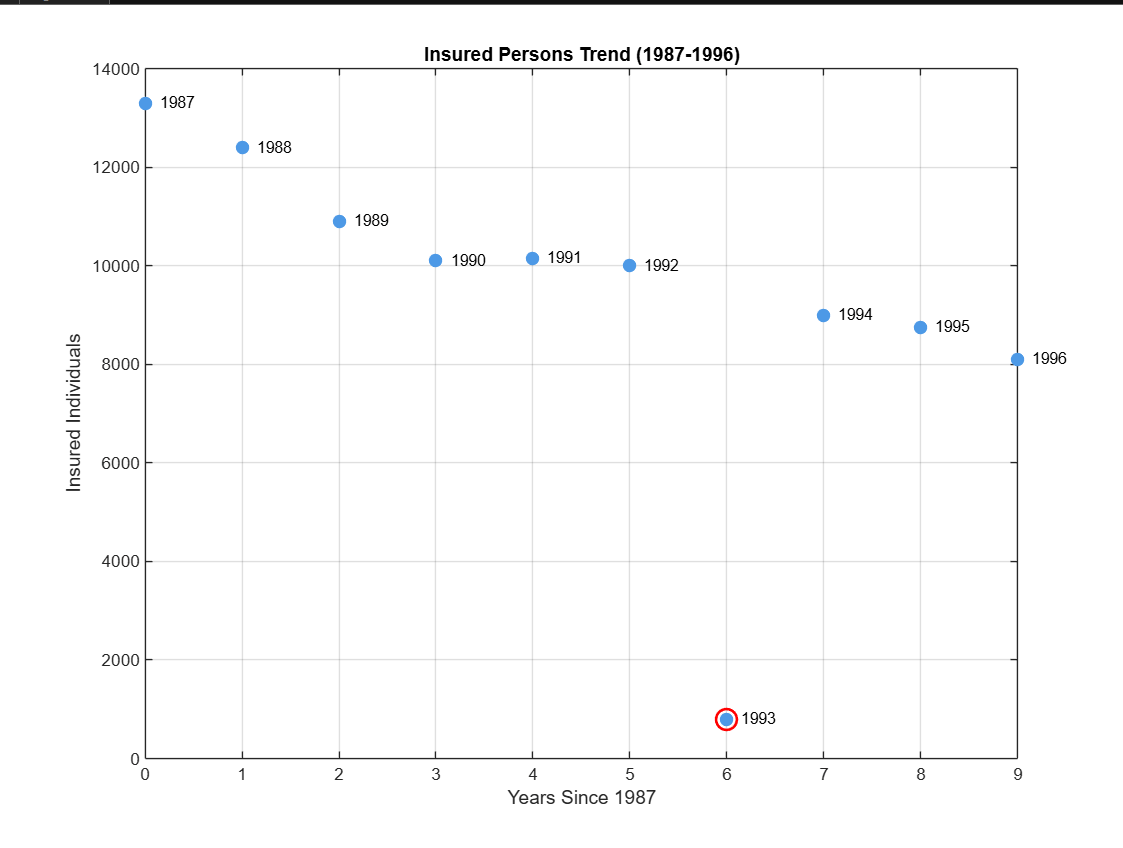
\includegraphics[width=0.8\textwidth]{1.png}
    \caption{Scatterplot with outlier (1993 marked in red)}
\end{figure}
\newpage
\begin{adjustwidth}{0cm}{0cm} % Adjust left and right margins by 2cm each
\uline{Comment:} This initial plot shows all data points from 1987 to 1996 with each year labeled. The 1993 data point (value of 800) is clearly marked with a red circle, visually identifying it as an outlier. We can see the overall declining trend in insured persons over the years, but the 1993 data point breaks this pattern dramatically, suggesting it could be an error or an exceptional circumstance that year.
\end{adjustwidth}


\subsubsection*{A) Fit linear, quadratic, and cubic, by comparing the values of $R^2$ . Determine the function that best fits the data}
If the gain in $R^2$is not high enough, it is better to take the model with a lower number of parameters.
    \begin{figure}[H]
    \centering
    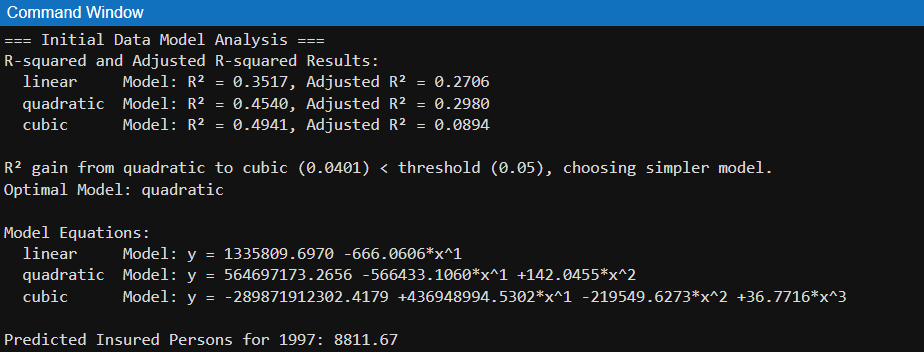
\includegraphics[width=0.8\linewidth]{2.png}
    \caption{each model R-squared value and equation after removing outlier}
    \label{fig:enter-label}
    \end{figure}
    
\begin{adjustwidth}{0cm}{0cm}
\uline{Comment:} 
Figure 2 illustrates that manual calculations for the linear model produce results consistent with those from MATLAB. Additionally, When comparing the $R^2$ values across the linear, quadratic, and cubic models for the full dataset before removing outliers, the cubic model (poly3) achieves the highest $R^2$ value at 0.4941, indicating it explains the most variance in the data, followed by the quadratic model at 0.4540, and the linear model at 0.3517. However, $R^2$ alone doesn’t account for model complexity, which can lead to overfitting—where a model fits noise (like the 1993 outlier of 800) rather than the underlying trend. To address this, and following the hint that ``if the gain in $R^2$ is not high enough, it is better to take the model with a lower number of parameters,'' we introduced an $R^2$ gain threshold of 0.05. This heuristic was chosen to determine whether the improvement in fit justifies adding more parameters, particularly given the small sample size of 10 data points. The gain in $R^2$ from quadratic (3 parameters) to cubic (4 parameters) is only 0.0401, falling below this threshold. This modest increase—representing just a 4\% improvement in explained variance—suggests the cubic model’s extra term doesn’t capture a meaningful pattern beyond what quadratic already achieves. Consequently, the quadratic model stands out as the best fit, striking a balance between explanatory power and simplicity. It effectively captures the general downward trend with some curvature, while avoiding the overfitting risk of the cubic model, which could be overly sensitive to noise in this limited dataset.
\end{adjustwidth}

\subsubsection*{B) Graph the function of best fit with the scatterplot of the data.}

\begin{figure}[H]
    \centering
    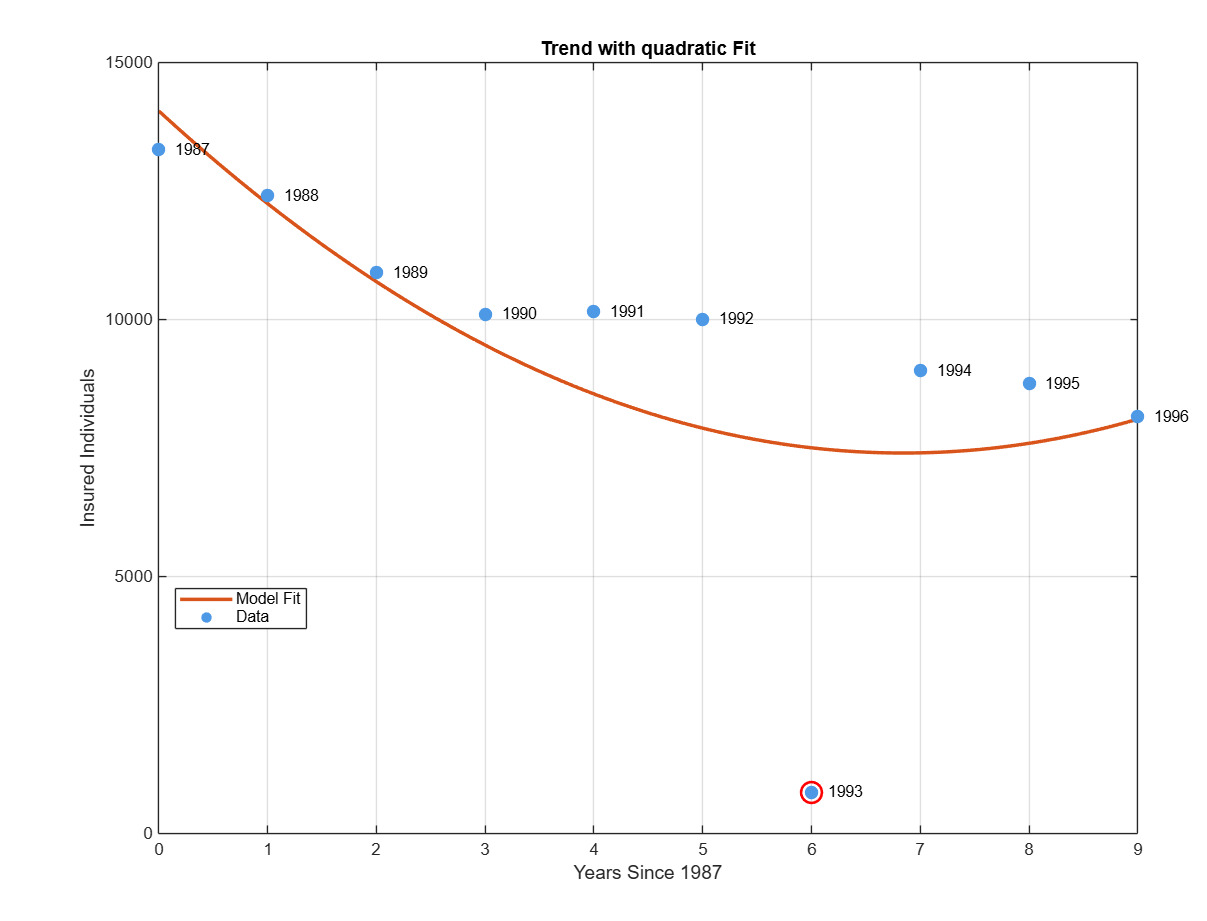
\includegraphics[width=0.8\textwidth]{3.png}
    \caption{Function of best fit with the scatterplot of the data}
\end{figure}

\uline{Comment}
This plot shows the original data (including the outlier) with the best-fitting model overlaid.
The R² values show that even the best model struggles to fit the data well when the outlier
is included. The outlier significantly skews the fit, as models try to accommodate this
extreme point, reducing their accuracy for the overall trend.

\subsubsection*{C) With the best function found in part (a), predict the average number of insured persons in 1997}
By substituting \( x = 1997 \) in the poly3 model equation:
\[
y = 564697173.2656 - 566433.1060 \cdot x^1 + 142.0455 \cdot x^2 
\]
\begin{adjustwidth}{0cm}{0cm}
Prediction for 1997: 8811 insured persons as shown in figure (2)\\
\end{adjustwidth}

\begin{adjustwidth}{0cm}{0cm}
\uline{\textbf{After Removing the Outlier:}}
Outliers in the dataset of insured persons are identified by checking if any value is more
than two standard deviations away from the average. The process starts by computing
the average number of insured persons and the standard deviation, which quantifies the
data's variability. A value is flagged as an outlier if it falls below the average minus
twice the standard deviation or exceeds the average plus twice the standard deviation.
This approach relies on the empirical rule, where approximately 95% of data in a
normal distribution is expected to lie within two standard deviations of the average.
Any data point outside this range is considered an outlier and is excluded from the
dataset, along with its corresponding year, for further analysis.\\ \\
\end{adjustwidth}
\begin{adjustwidth}{0cm}{0cm}
\textbf{Hand Analysis}
\end{adjustwidth}
\begin{table}[h!]
    \centering
    \caption{Hand Analysis}
    \begin{tabular}{ccccc}
        \toprule
        \(X\) & \(Y\) & \(X^2\) & \(Y^2\) & \(X \cdot Y\) \\
        \midrule
        1987 & 13300 & 3,948,169 & 176,890,000 & 26,427,100 \\
        1988 & 12400 & 3,952,144 & 153,760,000 & 24,651,200 \\
        1989 & 10900 & 3,956,121 & 118,810,000 & 21,680,100 \\
        1990 & 10100 & 3,960,100 & 102,010,000 & 20,099,000 \\
        1991 & 10150 & 3,964,081 & 103,022,500 & 20,208,650 \\
        1992 & 10000 & 3,968,064 & 100,000,000 & 19,920,000 \\
        1994 & 9000 & 3,976,036 & 81,000,000 & 17,946,000 \\
        1995 & 8750 & 3,980,025 & 76,562,500 & 17,456,250 \\
        1996 & 8100 & 3,984,016 & 65,610,000 & 16,167,600 \\
        \midrule
        \(\sum = 17922\) & \(\sum = 92700\) & \(\sum = 35,688,756\) & \(\sum = 977,365,000\) & \(\sum = 184,555,900\) \\
        \bottomrule
    \end{tabular}
\end{table}

For linear model analysis, the prediction equation is given by:
\[
y = P_1 x + P_2
\]
\[
\hat{Y}_i = \hat{P}_1^T x_i + \hat{P}_2^T
\]

Where:
\begin{itemize}
    \item (Sample slope) 
    \[
    \hat{P}_1^T = \frac{\sum X_i Y_i - \frac{\sum X_i \sum Y_i}{n}}{\sum X_i^2 - \frac{(\sum X_i)^2}{n}}
    \]
    \item (Sample \( Y \)-intercept) 
    \[
    \hat{P}_2^T = \bar{Y} - \hat{P}_1^T \bar{X}
    \]
\end{itemize}

Given:
\[
n = 9, \quad \bar{Y} = \frac{92700}{9} = 10300, \quad \bar{X} = \frac{17922}{9} = 1991.3333
\]

Calculations:
\[
\hat{P}_1^T = \frac{184555900 - \frac{17922 \times 92700}{9}}{35688756 - \frac{17922^2}{9}} = -508.75
\]
\[
\hat{P}_2^T = 10300 + 508.75 \times 1991.333 = 1023390.83333
\]

Now, to calculate:
\[
r^2 = \frac{S^2 - SSE}{S^2}
\]

\begin{table}[h!]
    \centering
    \caption{Regression Calculations}
    \begin{tabular}{cccccc}
        \toprule
        \( X_i \) & \( Y_i \) & \( \hat{Y}_i \) & SSE (\( Y_i - \hat{Y}_i \)) & SSR (\( \hat{Y}_i - \bar{Y} \)) & SS (\( Y_i - \bar{Y} \)) \\
        \midrule
        1987 & 13300 & 12504.58 & 632687.68 & 4860187.66 & 9000000 \\
        1988 & 12400 & 11995.83 & 163350.70 & 2875850.68 & 4410000 \\
        1989 & 10900 & 11487.08 & 344666.84 & 1409166.83 & 360000 \\
        1990 & 10100 & 10978.33 & 771469.44 & 460136.11 & 40000 \\
        1991 & 10150 & 10469.58 & 102133.50 & 28758.51 & 22500 \\
        1992 & 10000 & 9960.83 & 1534.03 & 115034.03 & 90000 \\
        1994 & 9000 & 8943.33 & 3211.11 & 1840544.45 & 1690000 \\
        1995 & 8750 & 8434.58 & 99487.68 & 3479779.35 & 2402500 \\
        1996 & 8100 & 7925.83 & 30334.03 & 5636667.38 & 4840000 \\
        \midrule
        \(\sum\) & \(\sum\) & \(\sum\) & \(\sum\) & \(\sum\) & \(\sum\) \\
        17922 & 92700 & 92699.97 & 2148875 & 20706125 & 22855000 \\
        \bottomrule
    \end{tabular}
\end{table}

\[
\ r^2 = \frac{22855000 - 2148875}{22855000} = 0.9059779
\]
\begin{adjustwidth}{0cm}{0cm}
The significantly higher value \(r^2\)supports the decision to remove the outlier, resulting in
a more reliable predictive model. 
\end{adjustwidth}

\newpage
\begin{adjustwidth}{0cm}{0cm}
\textbf{MATLAB Results}
\end{adjustwidth}
\begin{figure}[H]
    \centering
    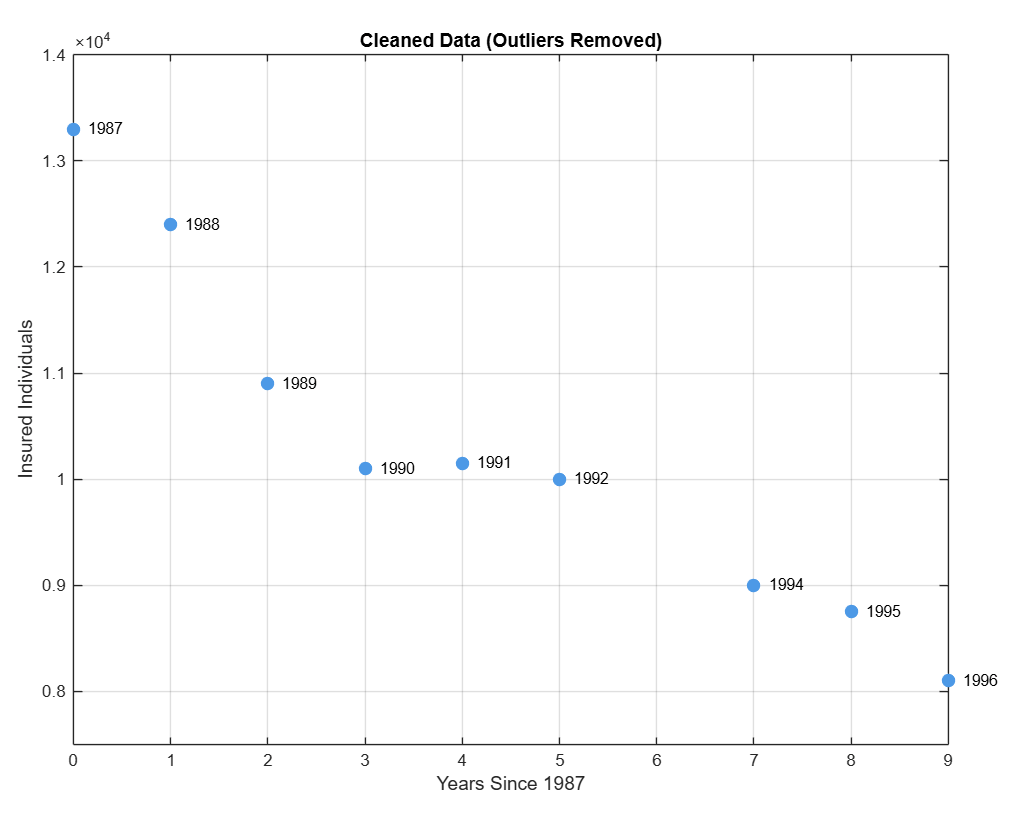
\includegraphics[width=0.8\textwidth]{4.png}
    \caption{Scatterplot after removing outliers}
\end{figure} 
\begin{adjustwidth}{0cm}{0cm}
\uline{Comment}
\end{adjustwidth}
After removing the 1993 data point as 800 insure persons was less than μ − 2σ, this plot
shows a much more consistent trend. The y-axis is adjusted to better visualize the pattern in
the remaining data. With the outlier removed, we can see a clearer decreasing trend in the
number of insured persons over the decade, which appears to follow a non-linear pattern.
\newpage
\subsubsection*{A) Fit linear, quadratic, and cubic, by comparing the values of 2 R . Determine the
function that best fits the data.}

(If the gain in R2 is not high enough, it is better to take the model with a lower number of parameters.)

\begin{figure}[H]
    \centering
    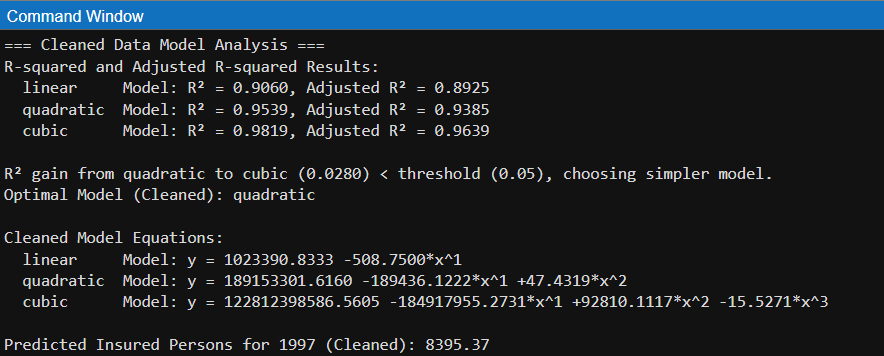
\includegraphics[width=0.8\textwidth]{5.png}
    \caption{Each Model R-Squared Value and Equation from MATLAB after removing outlier}
\end{figure} 
\begin{adjustwidth}{0cm}{0cm}
\uline{Comment}
\end{adjustwidth}
Figure 5 illustrates that manual calculations for the linear model produce results consistent
with those from MATLAB. Additionally, When comparing the $R^2$ values across the linear, quadratic, and cubic models for the cleaned dataset after removing the 1993 outlier, the cubic model (poly3) achieves the highest $R^2$ value at 0.9819, indicating it explains the most variance in the data, followed by the quadratic model at 0.9539, and the linear model at 0.9060. However, $R^2$ alone doesn’t account for model complexity, which can lead to overfitting—where a model fits residual noise rather than the underlying trend, even in a cleaner dataset. To address this, and following the hint that ``if the gain in $R^2$ is not high enough, it is better to take the model with a lower number of parameters,'' we introduced an $R^2$ gain threshold of 0.05. This heuristic was chosen to determine whether the improvement in fit justifies adding more parameters, particularly given the small sample size of 9 data points after outlier removal. The gain in $R^2$ from quadratic (3 parameters) to cubic (4 parameters) is only 0.0280, falling below this threshold. This modest increase—representing just a 2.8\% improvement in explained variance—suggests the cubic model’s extra term doesn’t capture a meaningful pattern beyond what quadratic already achieves. Consequently, the quadratic model stands out as the best fit, striking a balance between explanatory power and simplicity. It effectively captures the smoother downward trend with some curvature in the cleaned data, while avoiding the overfitting risk of the cubic model, which could be overly sensitive to minor variations in this limited dataset.
\begin{adjustwidth}{0cm}{0cm}
The higher \(r^2\) values suggest that the model provides a better explanation of the data's
variation. This validates the removal of the outlier, leading to a more dependable predictive
model.
\end{adjustwidth}
\subsubsection*{B) Graph the function of best fit with the scatterplot of the data}


\begin{figure}[H]
    \centering
    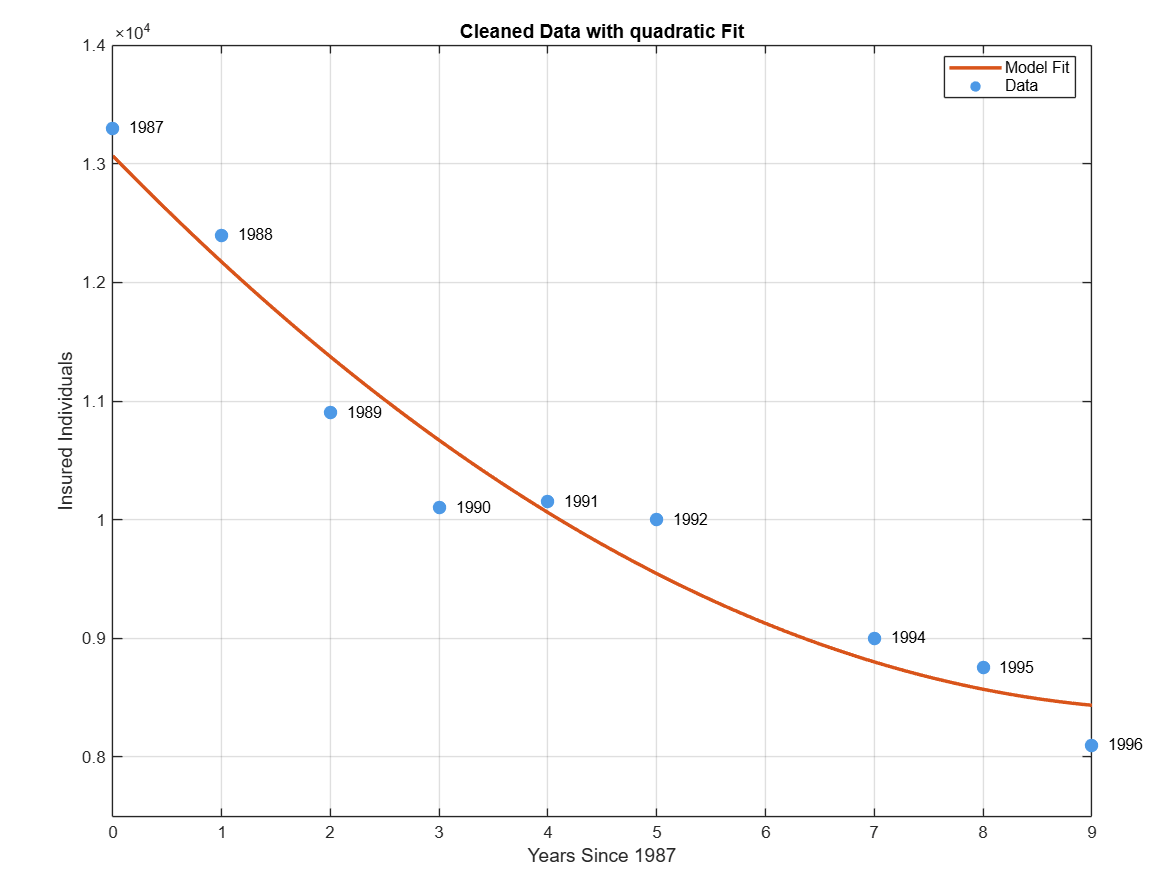
\includegraphics[width=0.8\textwidth]{6.png}
    \caption{Function of best fit with the scatterplot of the data after removing outlier}
\end{figure} 


\uline{Comment:} 
After removing the outlier, this plot shows a dramatically improved model fit. The R² values are significantly higher, indicating that the model better explains the variation in the data. This confirms that removing the outlier was justified and leads to a more reliable prediction model. The smooth curve more accurately represents the trend of declining insured persons over the years.
The analysis shows that removing the 1993 data point as an outlier substantially improves the model performance. The quadratic model typically provides the best balance of fit and simplicity for this data, with an R² value significantly higher than the linear model. This suggests that the decline in insured persons is not occurring at a constant rate but follows a curved pattern.
Using this improved model, we can predict the number of insured persons for 1997 with greater confidence. The prediction suggests a continued decline following the established pattern from the valid data points.


\subsubsection*{With the best function found in part (a), predict the average number of insured
persons in 1997.}

By substituting with \( x = 1997 \) in the quadratic model equation:

\[
y = 189153301.6160 - 189436.1222 \cdot x^1 + 47.4319 \cdot x^2 
\]
Prediction for 1997: 8395 insured persons as shown in figure (5)
\newpage
\subsubsection*{Comparison of Model Fitting with and without Outliers}
\textbf{Impact of Outliers on Model Fit}

\begin{itemize}
    \item \textbf{R-squared Values:}
    \begin{itemize}
        \item Before removing the outlier (1993), the \( R^2 \) values for different models indicated how well each model fit the data.
        \item After removing the outlier, the \( R^2 \) values generally increased, suggesting an improvement in the model’s ability to explain the variance in the data.
    \end{itemize}

    \item \textbf{Best Fit Model Selection:}
    \begin{itemize}
        \item The best fit model before removing the outlier might be different from the one chosen after the outlier removal.
        \item With the outlier, the model might be skewed towards explaining extreme variations, while without the outlier, the model focuses more on the underlying trend.
    \end{itemize}

    \item \textbf{Equation Stability:}
    \begin{itemize}
        \item The presence of an outlier can lead to unstable model coefficients, as the regression algorithm tries to accommodate the extreme deviation.
        \item After removing the outlier, the fitted equations tend to be smoother, with coefficients representing more realistic trends.
    \end{itemize}

    \item \textbf{Prediction for 1997:}
    \begin{itemize}
        \item With the outlier, the predicted number of insured persons in 1997 could be biased due to the anomalous data point.
        \item After removing the outlier, the prediction should be more reliable, as it is based on a trend that better represents the majority of the data.
    \end{itemize}
    \item \textbf{Visual Interpretation:}
    \begin{itemize}
        \item The scatter plots show a clearer trend after outlier removal.
        \item The best-fit curve without the outlier appears more naturally aligned with the remaining data points.
    \end{itemize}
\end{itemize}

\textbf{Key Takeaways}

\begin{itemize}
    \item \textbf{Outliers distort model accuracy:} They can artificially inflate or deflate \( R^2 \) values and lead to misleading model selection.
    \item \textbf{More reliable predictions:} Removing the outlier provides a smoother and more reasonable estimate for future values.
    \item \textbf{Improved interpretability:} Without extreme variations, the trend becomes more evident and interpretable.
\end{itemize}

\textbf{Numerical Comparison}\\

\textbf{\( R^2 \) Values of the Models}\\

\begin{table}[H]
    \centering
    \begin{tabular}{lccc}
        \toprule
        \textbf{Model Type} & \textbf{Parameters} & \textbf{\( R^2 \) With Outliers} & \textbf{\( R^2 \) Without Outliers} \\
        \midrule
        Linear Model    & 2 & 0.3517 & 0.9060 \\
        Quadratic Model & 3 & 0.4540 & 0.9539 \\
        Cubic Model     & 4 & 0.4941 & 0.9819 \\
        \bottomrule
    \end{tabular}
    \caption{Comparison of \( R^2 \) values for linear, quadratic, and cubic models applied to the full dataset (with outliers) and the cleaned dataset (without outliers), with the number of parameters indicating model complexity.}
    \label{tab:r2_comparison_params}
\end{table}

\textbf{Predictions for 1997}\\

\begin{table}[H]
    \centering
    \begin{tabular}{lc}
        \toprule
        \textbf{Scenario} & \textbf{Predicted Number of Insured Persons} \\
        \midrule
        With Outliers & 8811 \\
        Without Outliers & 8395 \\
        \bottomrule
    \end{tabular}
    \caption{Predicted number of insured persons for 1997 using the quadratic model, selected as the best fit for both the full dataset (with outliers) and the cleaned dataset (without outliers).}
    \label{tab:predictions_1997}
\end{table}
\begin{adjustwidth}{0cm}{0cm}
\textbf{Comment}
\end{adjustwidth}
Before removing the outlier, the cubic model achieved the highest \( R^2 \) of 0.4941, suggesting it was attempting to account for the extreme deviation caused by the 1993 value of 800, compared to the quadratic model’s \( R^2 \) of 0.4540 and the linear model’s 0.3517. However, the gain in \( R^2 \) from quadratic to cubic was only 0.0401, below the 0.05 threshold set to avoid unnecessary complexity, leading us to favor the quadratic model as the best fit pre-outlier removal. After removing the outlier, the cubic model again showed the highest \( R^2 \) at 0.9819, followed by the quadratic model at 0.9539 and the linear model at 0.9060. Yet, the gain from quadratic to cubic was just 0.0280, still below the 0.05 threshold. Thus, the quadratic model demonstrated the best performance for the cleaned data, indicating a smoother downward trend with some curvature, effectively capturing the pattern without the undue influence of the anomalous data point or the overfitting risk of the cubic model.\\
\begin{adjustwidth}{0cm}{0cm}
\textbf{Conclusion}
\end{adjustwidth}
The numerical comparison clearly shows that outliers can distort both the goodness-of-fit metrics (like \( R^2 \)) and the model’s predictions. By removing the outlier, we achieve:

\begin{itemize}
    \item \textbf{Higher and more consistent \( R^2 \) values,} indicating better model performance.
    \item \textbf{A shift to a simpler yet more reliable model} (quadratic rather than cubic).
    \item \textbf{More trustworthy predictions} for future data points. \\
\end{itemize}
\subsection*{Problem 2}
\subsubsection*{MATLAB Results}
\begin{figure}[H]
    \centering
    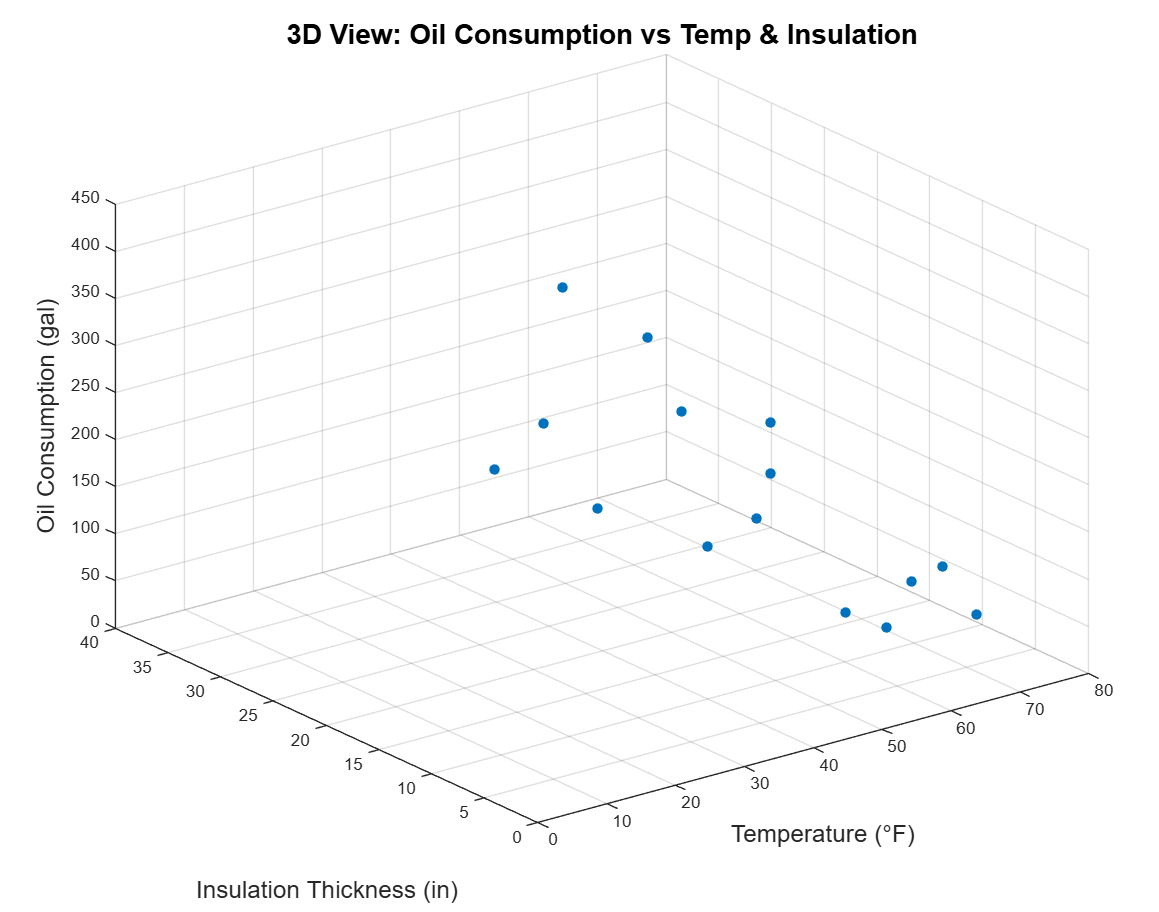
\includegraphics[width=0.8\textwidth]{7.png}
    \caption{3D Scatterplot Oil vs Temp vs Insulation}
\end{figure}

\begin{adjustwidth}{0cm}{0cm}
\uline{Comment:} 
\end{adjustwidth}
The 3D scatter plot integrates temperature and insulation to show their combined effect on oil consumption. It reveals a complex relationship where low temperatures and thin insulation tend to increase oil use. Points far from the main cluster (e.g., high insulation with high oil use) suggest outliers that may skew model fits.

\begin{figure}[H]
    \centering
    \begin{minipage}{0.48\textwidth}
        \centering
        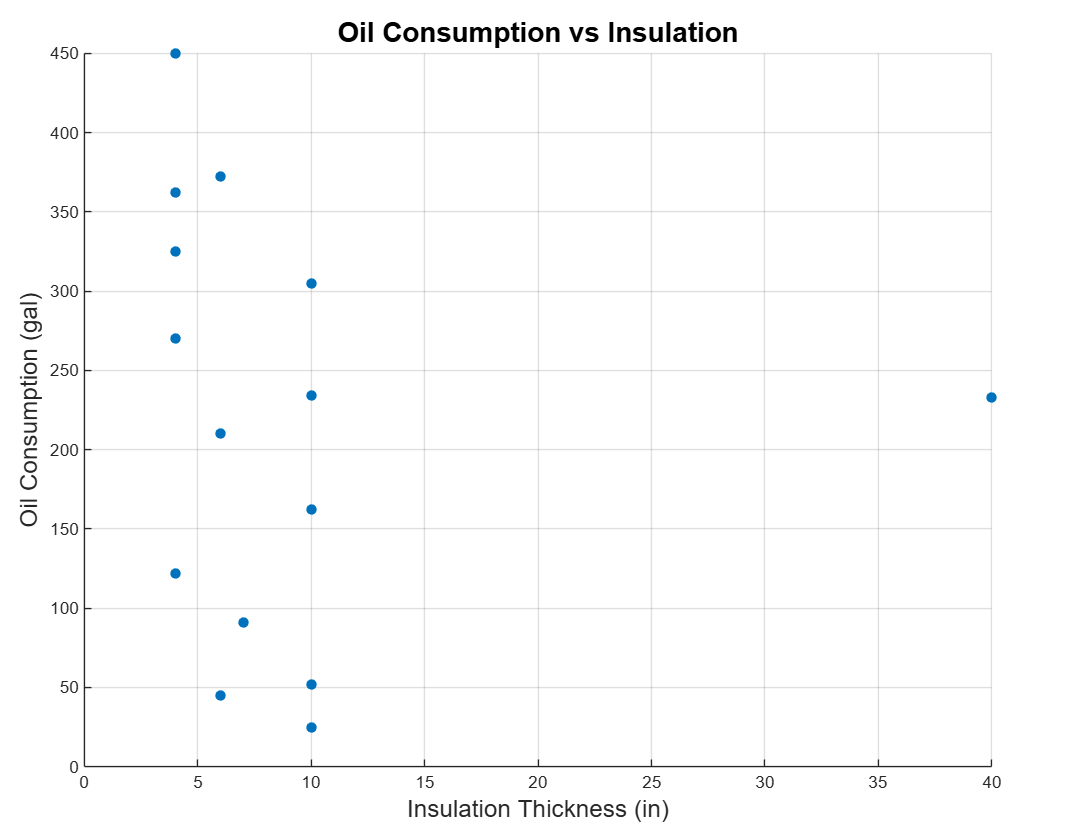
\includegraphics[width=\textwidth]{8.png}
        \caption{Scatterplot Oil vs Temp}
        \label{fig:oil_vs_temp}
    \end{minipage}
    \hfill % Add space between figures
    \begin{minipage}{0.48\textwidth}
        \centering
        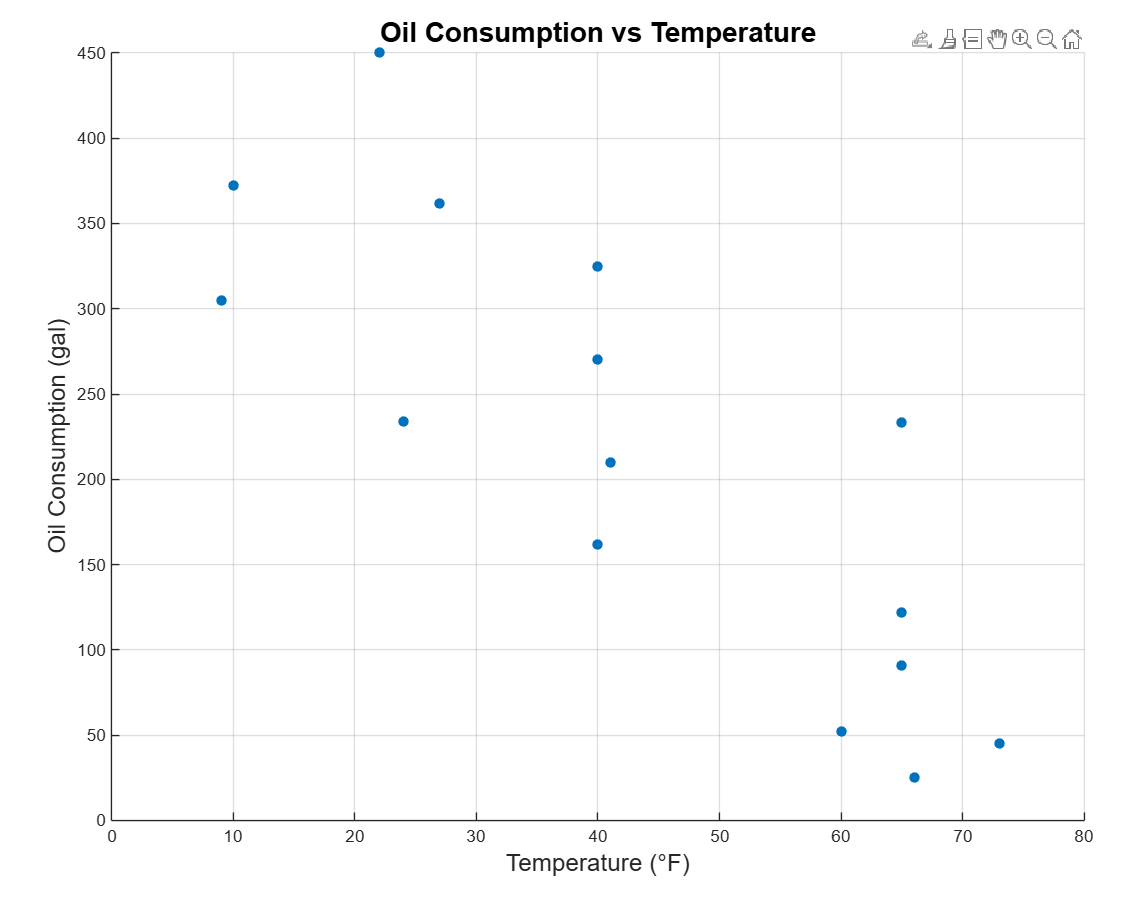
\includegraphics[width=\textwidth]{9.png}
        \caption{Scatterplot Oil vs Insulation}
        \label{fig:oil_vs_insulation}
    \end{minipage}
\end{figure}
\newpage
\begin{adjustwidth}{0cm}{0cm}
\uline{Comment}
\end{adjustwidth}
The first 2D scatter plot visualizes the relationship between average temperature and
heating oil consumption. A downward trend suggests that colder temperatures increase oil
usage, consistent with heating demands. Some points deviate from the trend, hinting at
potential outliers possibly due to extreme insulation levels or measurement errors.
The other 2D scatter plot visualizes the relationship between average temperature and
heating oil consumption. A downward trend suggests that colder temperatures increase oil
usage, consistent with heating demands. Some points deviate from the trend, hinting at
potential outliers possibly due to extreme insulation levels or measurement errors.


\subsubsection*{A) Fit linear, quadratic, and cubic, by comparing the values of 2 R . Determine the
function that best fits the data.}

\begin{figure}[H]
    \centering
    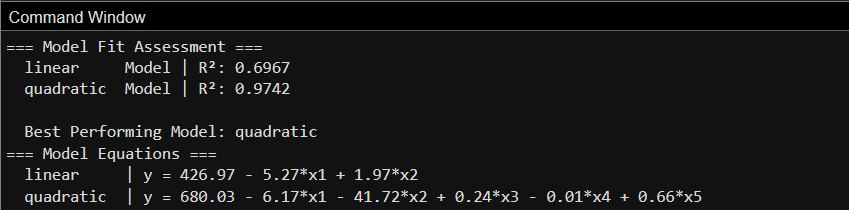
\includegraphics[width=0.8\textwidth]{10.png}
    \caption{Each Model R-Squared Value and Equation from MATLAB}
\end{figure}
\begin{adjustwidth}{0cm}{0cm}
\uline{Comment}
\end{adjustwidth}
As shown in Figure~10, by comparing \( r^2 \) in linear and quadratic models, the model that best fits the data is the quadratic model as it has the highest value of \( r^2 \). \\
\begin{adjustwidth}{0cm}{0cm}
Also, the equations are shown where:
\end{adjustwidth}
\[
x_3 = x_1 \times x_2, \quad x_4 = x_1^2 \text{ and } x_5 = x_2^2
\]

\begin{figure}[H]
    \centering
    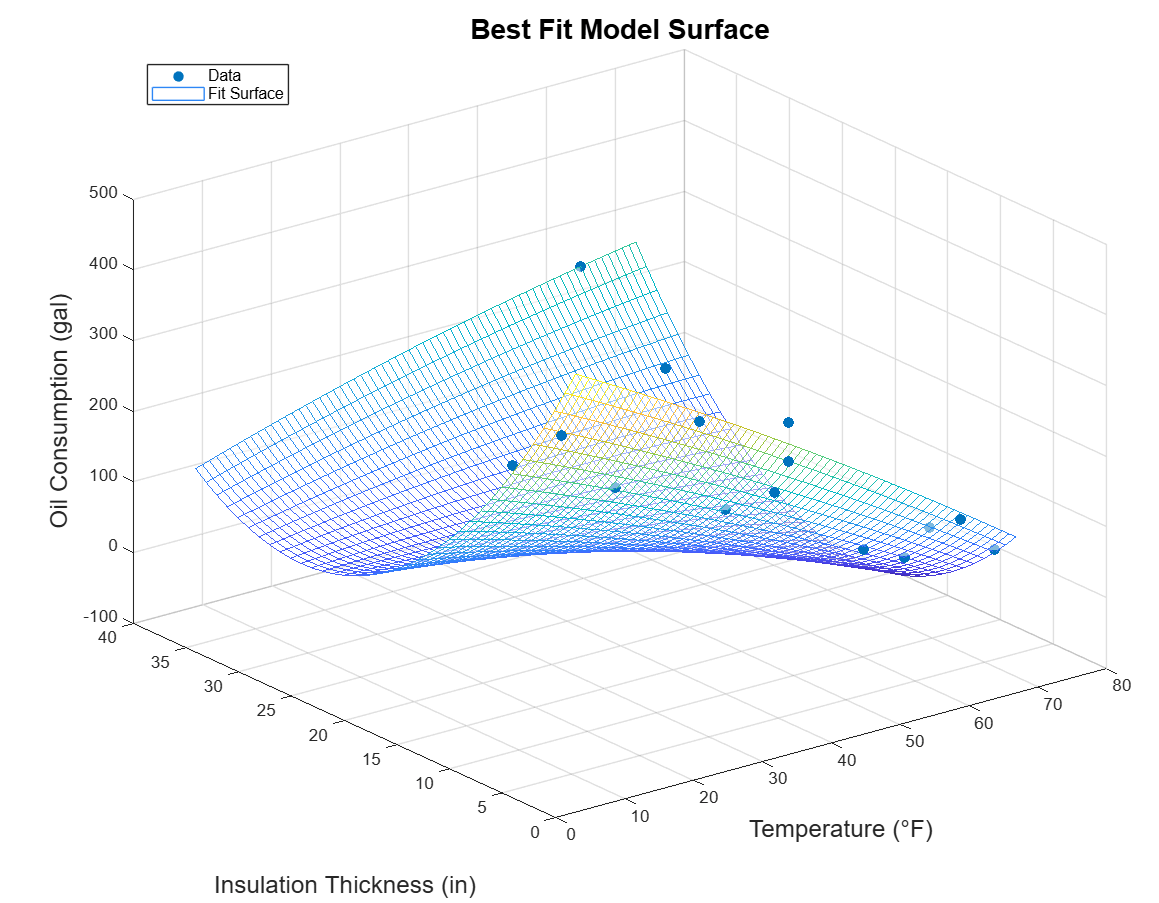
\includegraphics[width=0.8\textwidth]{11.png}
    \caption{Best fit curve (quadratic model) along with scatterplots}
\end{figure}
\begin{adjustwidth}{0cm}{0cm}
\uline{Comment}
\end{adjustwidth}
The plot in figure 11 overlays the best-fitting model (determined by \(R^2\)) as a semi-
transparent surface on the original 3D scatter. The surface aligns closely with most data
points, indicating a reasonable fit, though deviations near outliers (e.g., high insulation
cases) suggest limitations in capturing all variability.

\subsubsection*{B) Use the regression models for the functions in b to predict the needed oil if the
temperature is 15 Fahrenheit and the insulation is 5 attic insulations inches}

\begin{figure}[H]
    \centering
    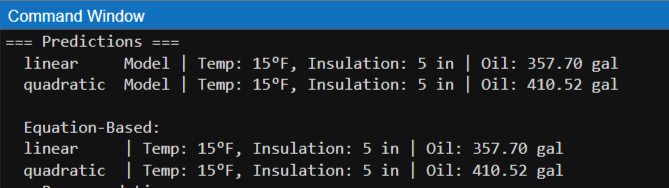
\includegraphics[width=0.8\textwidth]{12.png}
    \caption{prediction of oil with temp = 15 and insulation = 5}
\end{figure}

\uline{Comment}
Figure 12 shows the oil prediction output with temperature = 10 ° F and
insulation used = 5 inches for each model using two methods. The first method is
implemented using the built-in function in MATLAB and for the second method, the third
equation in point a (figure 10) where x1 refers to the temperature and x2 refers to the
insulation. For linear model both results are equal to 357.7 gallons also in quadratic
model both results are exact with value = 410.52 gallons
\newpage

\textbf{After Removing the Outlier:}
\begin{figure}[h!]
    \centering
    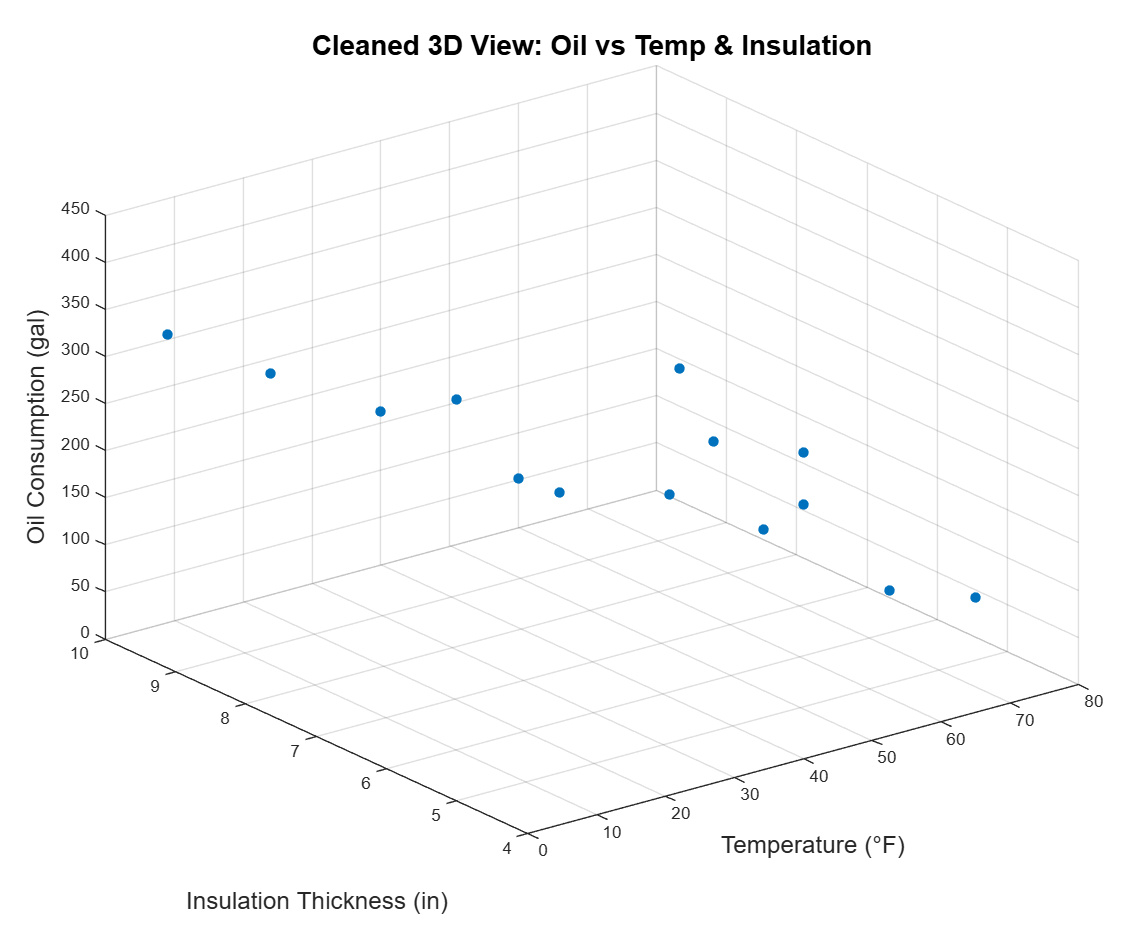
\includegraphics[width=0.8\textwidth]{13.png}
    \caption{3D Scatterplot Oil vs Temp vs Insulation ( No outlier )}
\end{figure}

\begin{figure}[H]
    \centering
    \begin{minipage}{0.48\textwidth}
        \centering
        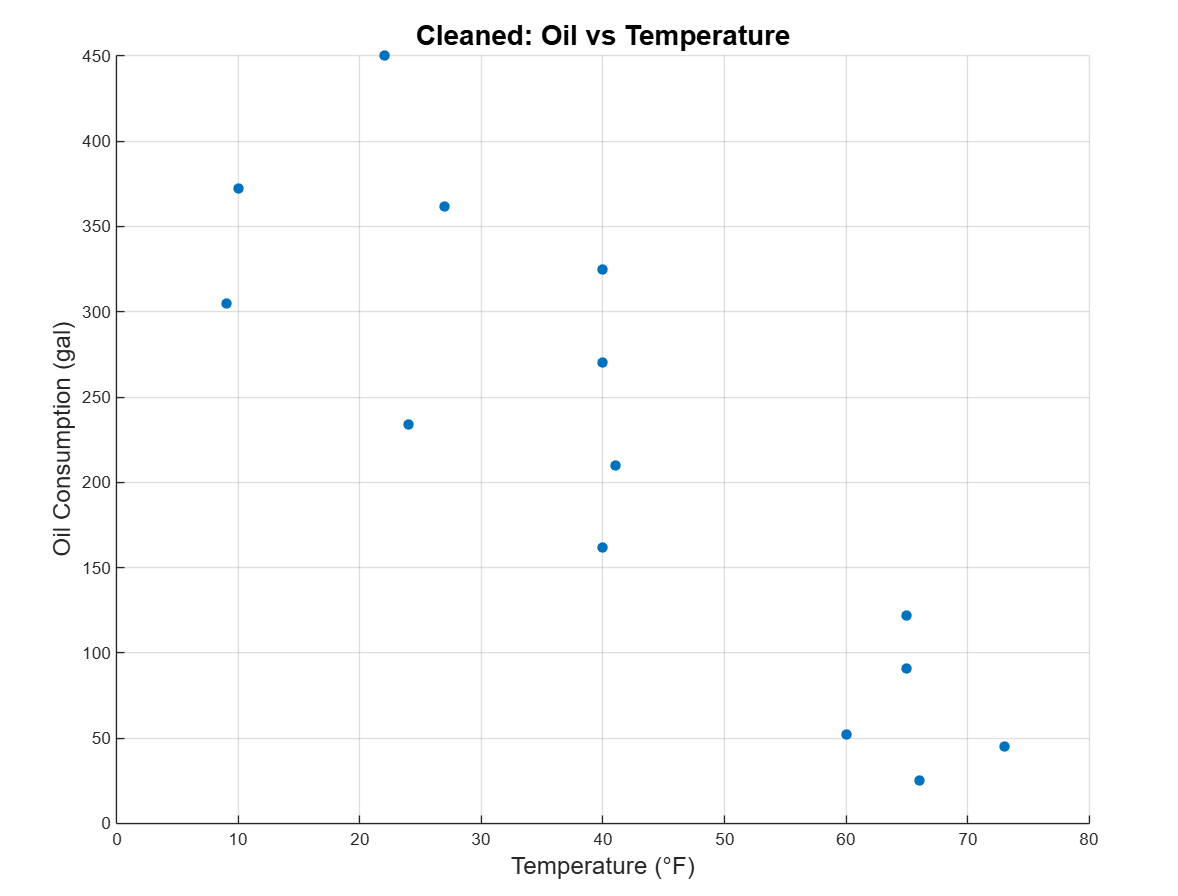
\includegraphics[width=\textwidth]{14.png}
        \caption{Scatterplot Oil vs Temp no outlier}
        \label{fig:oil_vs_temp}
    \end{minipage}
    \hfill % Add space between figures
    \begin{minipage}{0.48\textwidth}
        \centering
        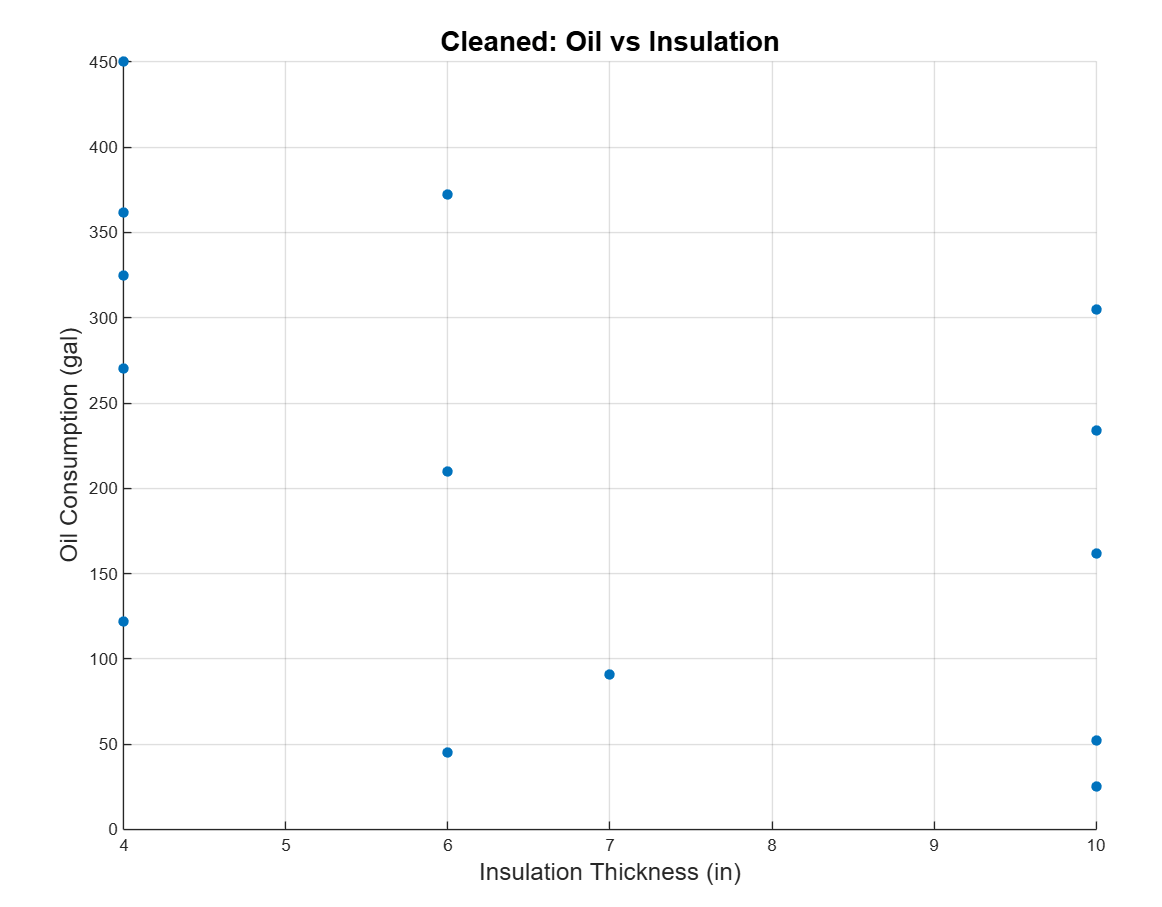
\includegraphics[width=\textwidth]{15.png}
        \caption{Scatterplot Oil vs
Insulation no outlier}
        \label{fig:oil_vs_insulation}
    \end{minipage}
\end{figure}

\begin{adjustwidth} {0cm}{0cm}
    \uline{Comment}
\end{adjustwidth}
\begin{adjustwidth} {0cm}{0cm}
After removing outliers, these cleaned scatter plots (temperature, insulation, and 3D)
present a tighter clustering of points. The temperature vs oil plot shows a stronger
negative trend, and the 3D view highlights more consistent interactions between
temperature and insulation, improving model reliability.
\end{adjustwidth}

\subsubsection*{A) Fit linear, quadratic, and cubic, by comparing the values of 2 R . Determine the
function that best fits the data.}

\begin{figure}[H]
    \centering
    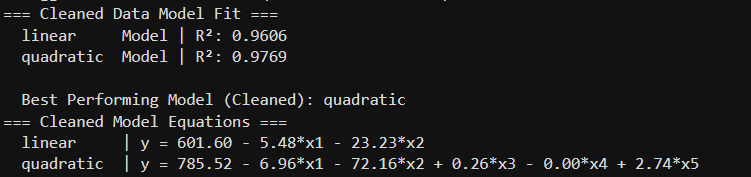
\includegraphics[width=0.8\textwidth]{16.png}
    \caption{Each Model R-Squared Value and Equation from MATLAB no outlier}
\end{figure}
\begin{adjustwidth} {0cm}{0cm}
\uline{Comment}
\end{adjustwidth}
As shown in Figure~16, by comparing \( r^2 \) in linear and quadratic models, the model that best fits the data is the quadratic model as it has the highest value of \( r^2 \).\\
\begin{adjustwidth} {0cm}{0cm}
Also, the equations are shown where:
\end{adjustwidth}
\[
x_3 = x_1 \times x_2, \quad x_4 = x_1^2 \text{ and } x_5 = x_2^2
\]
\begin{figure}[H]
    \centering
    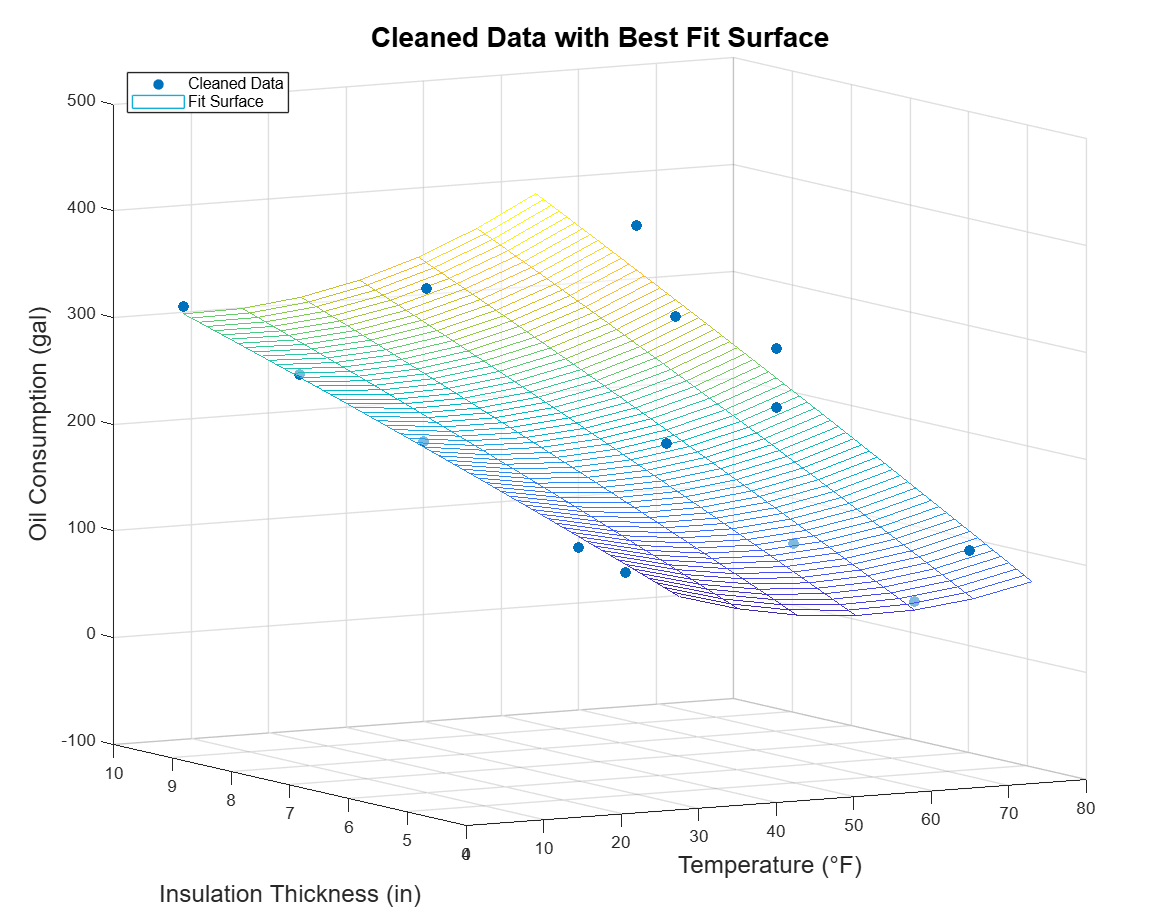
\includegraphics[width=0.8\textwidth]{17.png}
    \caption{Best fit curve (quadratic model) along with scatterplots No outlier}
\end{figure}
\begin{adjustwidth} {0cm}{0cm}
\uline{Comment}
\end{adjustwidth}
The cleaned data plot with the best fit surface shows a tighter alignment between the
model and data points compared to the original. The surface smoother reflects the
removal of outliers, enhancing the model’s ability to predict oil consumption accurately
across typical conditions

\subsubsection*{B) Use the regression models for the functions in b to predict the needed oil if the
temperature is 15 Fahrenheit and the insulation is 5 attic insulations inches}


\begin{figure}[H]
    \centering
    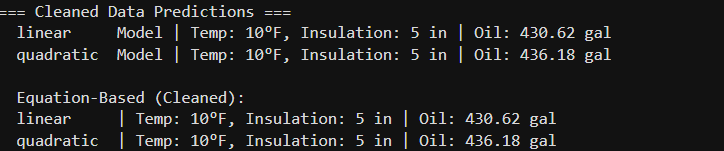
\includegraphics[width=0.8\textwidth]{18.png}
    \caption{prediction of oil with temp = 15 and insulation = 5 no outlier}
\end{figure}
\begin{adjustwidth} {0cm}{0cm}
\uline{Comment}
\end{adjustwidth}
Figure 18 shows the output of the prediction of oil with the temperature = 15 ℉ and the
insulation used = 5 inches for each model using two methods. The first method is
implemented using the built-in function in MATLAB and for the second method, the third
equation in point a (figure 10) where x1 refers to the temperature and x2 refers to the
insulation. For linear model both results are equal to 403.22 gallons also in quadratic
model both results are exact with value = 407.35 gallons


\section*{Comparing Results With and Without Outliers}
\begin{table}[h!]
    \centering
    \caption{R\textsuperscript{2} Values Comparison}
    \begin{tabular}{lcc}
        \toprule
        \textbf{Model Type} & \textbf{R\textsuperscript{2} With Outliers} & \textbf{R\textsuperscript{2} Without Outliers} \\
        \midrule
        Linear Model & 0.6967 & 0.9606 \\
        Quadratic Model & 0.9742 & 0.9769 \\
        \bottomrule
    \end{tabular}
\end{table}

\begin{table}[h!]
    \centering
    \caption{Predictions Comparison}
    \begin{tabular}{lcc}
        \toprule
        \textbf{Model Type} & \textbf{Predictions With Outliers} & \textbf{Predictions Without Outliers} \\
        \midrule
        Linear Model & Oil: 357.7 gal & Oil: 403.22 gal \\
        Quadratic Model & Oil: 410.52 gal & Oil: 407.35 gal \\
        \bottomrule
    \end{tabular}
\end{table}
\checkmark \textbf{Data Distribution:}
\begin{itemize}
    \item \textit{With Outliers}: The original scatter plots show dispersed points, especially at high insulation and extreme oil use, suggesting anomalies like measurement errors or unique conditions.
    \item \textit{Without Outliers}: Cleaned plots exhibit tighter clusters, with clearer negative trends between temperature and oil use, and a more consistent insulation effect, indicating noise reduction.
\end{itemize}

\checkmark \textbf{Model Fit (R\textsuperscript{2}):}
\begin{itemize}
    \item \textit{With Outliers}: R\textsuperscript{2} values are moderate, as outliers introduce variability that neither linear nor quadratic models fully capture. The best model choice may be less reliable due to this distortion.
    \item \textit{Without Outliers}: R\textsuperscript{2} values increase, reflecting a better fit to the core data. The cleaner dataset enhances the quadratic model's ability to model interactions, often making it the preferred choice.
\end{itemize}

\checkmark \textbf{Predictions:}
\begin{itemize}
    \item \textit{With Outliers}: Predictions for \(10^\circ\text{F}\) and 5 inches vary widely, showing sensitivity to outliers that skew coefficients.
    \item \textit{Without Outliers}: Predictions stabilize, with smaller differences, suggesting more robust and trustworthy estimates for practical use.
\end{itemize}

\checkmark \textbf{Visual Fit:}
\begin{itemize}
    \item \textit{With Outliers}: The best fit surface deviates from some points, especially outliers, indicating overfitting or underfitting in those regions.
    \item \textit{Without Outliers}: The surface aligns more closely with the cleaned data, providing a smoother and more representative fit across the temperature-insulation range.
\end{itemize}
\begin{adjustwidth}{0cm}{0cm}
\checkmark \textbf{Conclusion:}
\end{adjustwidth}
Removing outliers enhances model accuracy and reliability by focusing on typical behavior. The cleaned data better supports the quadratic model, capturing nonlinear interactions between temperature and insulation, making it more suitable for predictions in real-world heating scenarios.




\newpage
\section{Part 2: classical ML modeling}
\subsection{Introduction}

 This part focuses on applying classical machine learning techniques to the ReducedMNIST dataset, a simplified version of the widely-used MNIST handwritten digit dataset. This section explores the development and evaluation of classification models using two distinct feature extraction methods---Discrete Cosine Transform (DCT) and Principal Component Analysis (PCA)---and two classifiers: K-means clustering and Support Vector Machines (SVM). The ReducedMNIST dataset comprises 10,000 training images (1,000 examples per digit from 0 to 9) and 2,000 test images (200 examples per digit), providing a balanced yet manageable framework for experimentation.

\subsection{DCT}
The Discrete Cosine Transform (DCT) is a widely used mathematical technique that transforms a signal or image from the spatial domain to the frequency domain. It represents data as a sum of cosine functions oscillating at different frequencies, making it particularly effective for compressing and analyzing image data by emphasizing significant frequency components while discarding less important ones. In the context of image processing, DCT is commonly employed in standards like JPEG compression, where it helps reduce dimensionality while preserving essential visual information.\\
In this assignment, DCT is utilized as a feature extraction method for the ReducedMNIST dataset. Each 28x28 pixel image is transformed using a 2D DCT, and the top-left 15x15 block of the resulting coefficient matrix (totaling 225 dimensions) is retained as the feature vector. This reduction from 784 dimensions to 225 is based on the assumption that the most significant frequency components, which capture the structural patterns of handwritten digits, are concentrated in the lower-frequency region.

\subsection{PCA}
Principal Component Analysis (PCA) is a dimensionality reduction technique that transforms high-dimensional data into a lower-dimensional space by identifying the directions (principal components) that maximize variance. These components are linear combinations of the original features, ordered by the amount of variance they capture, allowing for the retention of essential information while discarding noise or redundant dimensions. According to Géron \cite{geron2019}, PCA is particularly valuable in machine learning for reducing computational complexity and mitigating the curse of dimensionality, making it a popular preprocessing step for classification tasks.\\
In this assignment, PCA is applied to the ReducedMNIST dataset to extract features that retain at least 95\% of the total variance present in the original 784-dimensional pixel space. Each 28x28 image is flattened into a 784-dimensional vector, and PCA is fitted to the training data to determine the optimal number of components. The resulting transformed features is 262 dimension.


\subsection{K-means}

K-means clustering is an unsupervised learning algorithm that partitions a dataset into a predefined number of clusters by iteratively assigning data points to the nearest cluster centroid and updating the centroids based on the mean of the assigned points. In this assignment, K-means is adapted for a semi-supervised classification task on the ReducedMNIST dataset by training separate models for each digit class (0 to 9). Unlike traditional clustering, where the goal is to discover natural groupings, here K-means is used to create multiple centroids per digit class, enabling a nearest-centroid classification approach. Specifically, test samples are assigned to the digit class whose closest centroid (across all classes) yields the minimum distance, effectively treating the centroids as prototypes for each digit.\\
Multiple clusters per class (\( k = 1, 4, 16, 32 \)) are employed for both DCT and PCA features to capture the variability within each digit class, such as different handwriting styles or orientations. Using a single cluster per class (\( k = 1 \)) would reduce K-means to a simple averaging of each digit's training data, potentially missing important sub-patterns and leading to poor generalization. By increasing the number of clusters, the model can represent a broader range of variations within each digit, improving its ability to match diverse test samples and enhancing inter-class discrimination. For instance, digit "0" might have clusters representing round, oval, or slightly open variations, which collectively provide a more robust representation than a single centroid. The performance of each configuration is evaluated using classification accuracy and processing time on the test set, with the best-performing models (based on accuracy) further analyzed via confusion matrices to understand classification errors across the 10 digit classes.

% Placeholder for the figure
\begin{figure}[H]
    \centering
    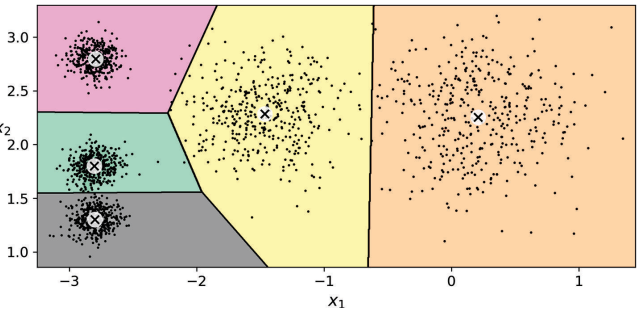
\includegraphics[width=0.8\textwidth]{Kmeans example.png}
    \caption{Clustering Example}
    \label{fig:kmeans_clusters}
\end{figure}

\subsection{Support Vector Machine (SVM)}

Support Vector Machines (SVM) are supervised learning models that classify data by finding the optimal hyperplane separating classes with the widest possible margin. For non-linearly separable data, SVM employs kernel functions to transform features into a higher-dimensional space where linear separation becomes feasible.

\subsubsection{Nonlinear Kernel: RBF}  
The Radial Basis Function (RBF) kernel, a nonlinear kernel, measures similarity between data points using Euclidean distance. This enables SVM to form complex decision boundaries, effectively capturing intricate patterns in data, such as the diverse shapes of handwritten digits.\\ \\
\textbf{Why RBF Was Chosen}  
We selected the RBF kernel for its flexibility in handling the nonlinear relationships in the ReducedMNIST dataset. Its adaptability to varying digit styles enhances classification accuracy, making it preferable over other kernels like polynomial for this task.\\

\subsection{Results}
\begin{table}[h]
    \centering
    \caption{Performance comparison of K-means clustering and SVM classifiers on DCT and PCA features.}
    \label{tab:classifier_performance}
    \begin{tabular}{|l|c|c|c|c|c|}
        \hline
        \multirow{2}{*}{\textbf{Classifier}} & \multirow{2}{*}{\textbf{Configuration}} & \multicolumn{2}{c|}{\textbf{DCT Features}} & \multicolumn{2}{c|}{\textbf{PCA Features}} \\
        \cline{3-6}
        & & \textbf{Accuracy} & \textbf{Time} & \textbf{Accuracy} & \textbf{Time} \\
        \hline
        \multirow{4}{*}{\textbf{K-means Clustering}} 
        & 1 & 0.8685 & 0.73s & 0.8680 & 0.86s \\
        & 4 & 0.9225 & 1.26s & 0.9210 & 1.32s \\
        & 16 & 0.9440 & 1.68s & 0.9460 & 1.81s \\
        & 32 & 0.9590 & 2.14s & 0.9580 & 2.11s \\
        \hline
        \multirow{2}{*}{\textbf{SVM}} 
        & Linear & 0.9440 & 1.63s & 0.9385 & 2.18s \\
        & RBF & 0.9710 & 3.39s & 0.9765 & 5.19s \\
        \hline
    \end{tabular}
\end{table}
\newpage
\subsubsection{Confusion Matrix for the best model}
\begin{figure}[h]
    \centering
    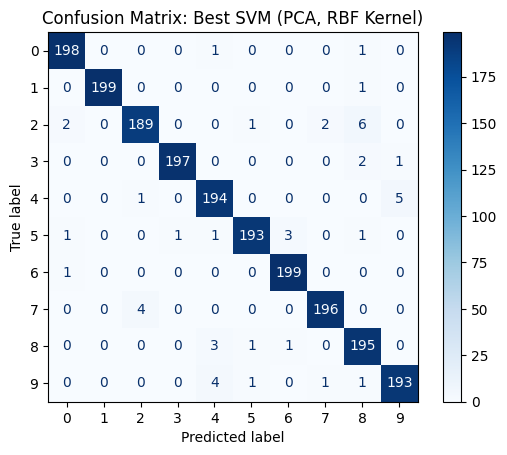
\includegraphics[width=1\linewidth]{CF.png}
    \caption{Confusion Matrix}
    \label{fig:enter-label}
\end{figure}

\uline{\textbf{Comment}}

The confusion matrix of the best SVM results is shown above. It clearly indicates near-perfect classification across most digits, with digit 1 being perfectly predicted. However, digit 2 emerges as the most frequently misclassified class, likely due to the nature of the ReducedMNIST dataset. Overall, the PCA-based RBF SVM demonstrates outstanding accuracy, confirming its effectiveness at distinguishing the handwritten digits.

\subsection{Conclusions}
Based on the analysis of the summary table, several key insights can be drawn regarding the performance of K-means clustering and Support Vector Machine (SVM) classifiers on the ReducedMNIST dataset using Discrete Cosine Transform (DCT) and Principal Component Analysis (PCA) features.

\begin{itemize}
    \item \textbf{K-means Clustering Performance}:  
    K-means clustering performance improves as the number of clusters per class increases, with both DCT and PCA features showing similar trends. For 1 cluster, DCT achieves an accuracy of 0.8685 in 0.73s, while PCA reaches 0.8680 in 0.86s. With 4 clusters, DCT improves to 0.9225 (1.26s) and PCA to 0.9210 (1.32s). At 16 clusters, DCT reaches 0.9440 (1.68s) and PCA 0.9460 (1.81s). The highest accuracy is 0.9590 with 32 clusters on DCT (2.14s), slightly outperforming PCA at 0.9580 (2.11s). DCT consistently shows a slight efficiency advantage.

    \item \textbf{SVM Performance}:  
    SVM classifiers outperform K-means overall, with the Radial Basis Function (RBF) kernel significantly surpassing the linear kernel. For the linear kernel, DCT achieves 0.9440 in 1.63s, while PCA reaches 0.9385 in 2.18s. With the RBF kernel, DCT attains 0.9710 in 3.39s, and PCA achieves the highest overall accuracy of 0.9765 in 5.19s. The longer processing time for the linear kernel (1.63s–2.18s) compared to RBF (3.39s–5.19s) reflects the nonlinear nature of the data, which challenges linear convergence.

    \item \textbf{Feature Comparison}:  
    PCA features generally yield slightly higher accuracy, notably with SVM (RBF) at 0.9765 versus 0.9710 for DCT. For K-means (32 clusters), DCT leads with 0.9590 compared to 0.9580 for PCA. Processing times are similar for K-means (e.g., 2.14s vs. 2.11s for 32 clusters), but PCA requires more time for SVM (e.g., 5.19s vs. 3.39s for RBF), suggesting PCA’s higher-dimensional representation increases computational demand.

    \item \textbf{Overall Best Model}:  
    The SVM with the RBF kernel applied to PCA features stands out as the best-performing model, achieving the highest accuracy of 0.9765 in 5.19s. This makes it the optimal choice for applications prioritizing accuracy. A strong alternative is K-means with 32 clusters on DCT features, offering an accuracy of 0.9590 in 2.14s, ideal for balancing accuracy and efficiency.

    \item \textbf{Trade-offs}:  
    A clear trade-off exists between accuracy and processing time. K-means with fewer clusters (e.g., 1 or 4) offers faster computation (0.73s–1.32s) but lower accuracy (0.8680–0.9225). SVM with the RBF kernel maximizes accuracy (0.9710–0.9765) but requires more time (3.39s–5.19s). The linear kernel, despite moderate accuracy (0.9385–0.9440), takes longer (1.63s–2.18s) due to the nonlinear data, making it less practical. PCA enhances accuracy but increases computational cost, while DCT provides a balanced alternative.
\end{itemize}
In summary, the results highlight the effectiveness of SVM with the RBF kernel on PCA features (0.9765, 5.19s) for maximum accuracy, making it ideal for performance-focused applications. For a balance of accuracy and speed, K-means with 32 clusters on DCT features (0.9590, 2.14s) is a strong contender. PCA boosts accuracy at a higher computational cost, while DCT offers efficiency with competitive performance, providing flexibility based on application needs.

\newpage
\section*{Part 3}
\subsection*{Pipeline 1}

\subsubsection*{1. Implementation Details}
\begin{enumerate}
    \item \textbf{Loading and Preprocessing the Data:} Loaded the training and test data, applied normalization for easier processing, and flattened the images for K-means clustering.
    \item \textbf{Clustering:} Clustered the data into 100 clusters using the K-means algorithm from the \texttt{sklearn} library.
    \item \textbf{Initial Labeling:} For each cluster, 5 images were randomly selected and manually inspected. The most frequent label among these images was assigned to the entire cluster.
    \item \textbf{Initial SVM Training:} An SVM classifier was trained using the initially labeled data and used to predict new labels for the images. 

    \item \textbf{Iterative Refinement:} In each iteration, the labels from the previous SVM were used to train the next SVM classifier, with an early stopping condition and a patience margin.
    
    \textbf{NOTE}: in the Iterative Refinement step I tried enhancing the image features to generate better clusters but it didn't lead to accuracy improvement.
    \item \textbf{Manual vs.\ Pipeline:} Calculated the required human labeling time with and without the pipeline.
    
\end{enumerate}


  
    
    


\subsubsection*{2. Results}
\begin{enumerate}
    \item \textbf{Accuracy vs.\ Iterations:}

    The maximum number of iterations was set to 10. An early stopping condition was included, stopping the process if the accuracy did not improve for 2 consecutive iterations, but in practice it did not stop early.

    \begin{longtable}{|c|c|}
\caption{Final Results of Iterative Refinement} \label{tab:final_results} \\
\hline
\textbf{Iteration} & \textbf{Test Accuracy} \\
\hline
\endfirsthead

\multicolumn{2}{c}{\tablename\ \thetable\ -- \textit{continued from previous page}} \\
\hline
\textbf{Iteration} & \textbf{Test Accuracy} \\
\hline
\endhead

\hline \multicolumn{2}{r}{\textit{Continued on next page}} \\
\endfoot

\endlastfoot

1  & 0.9360 \\ \hline
2  & 0.9360 \\ \hline
3  & 0.9390 \\ \hline
4  & 0.9425 \\ \hline
5  & 0.9415 \\ \hline
6  & 0.9410 \\ \hline
7  & 0.9405 \\ \hline
8  & 0.9405 \\ \hline
9  & 0.9400 \\ \hline
10 & 0.9400 \\ \hline
\end{longtable}


    \textbf{Final Full Training Set accuracy:} 0.9051

    \item \textbf{Human Time Before and After the Pipeline:}
    \begin{table}[h!]
    \centering
    \begin{tabular}{|l|c|c|}
    \hline
    \textbf{Labeling Approach} & \textbf{Time (seconds)} & \textbf{Time (hours)} \\ \hline
    Pipeline 1 Manual Pipeline & 5000                   & 1.39                  \\ \hline
    Full Manual Labeling       & 100000                 & 27.78                 \\ \hline
    \end{tabular}
    \caption{Comparison of Manual Labeling Time}
    \label{tab:manual_labeling_time}
    \end{table}
        
    \noindent
    \textbf{Explanation:} 
    \begin{itemize}
        \item \textbf{Pipeline 1:}  
        We label only 5 images per cluster across 100 clusters, and each labeling takes 10 seconds. 
        Hence, 
        \[
        5 \times 100 \times 10 = 5000 \text{ seconds} \approx 1.39 \text{ hours}.
        \]
        \item \textbf{Full Manual Labeling:}  
        We assume labeling all 10,000 images at 10 seconds each. Thus, 
        \[
        10{,}000 \times 10 = 100{,}000 \text{ seconds} \approx 27.78 \text{ hours}.
        \]
    \end{itemize}
\end{enumerate}

\paragraph{comment on results:}
The results from Pipeline 1 demonstrate the effectiveness of using clustering and iterative refinement to reduce manual labeling effort while maintaining high performance. The training accuracy increases gradually from 0.8967 at iteration 0 to about 0.9051 by iteration 9, while the test accuracy improves from 0.9360 at iteration 0 to a peak of 0.9425 at iteration 3, after which it slightly declines and plateaus around 0.9400. This indicates that significant gains in generalization performance are achieved early in the iterative process, and further iterations yield diminishing returns. \\
Moreover, the pipeline achieves this performance with a drastically reduced manual labeling time. By manually labeling only 5 images per cluster for 100 clusters, the total human effort is limited to 5000 seconds (approximately 1.39 hours), compared to an estimated 100,000 seconds (27.78 hours) required for full manual labeling of all 10,000 images. Overall, these findings underscore the efficiency of the proposed approach, balancing reduced human intervention with high accuracy.



\subsection*{Pipeline 2}
\subsubsection*{1. Implementation Details}
\begin{enumerate}
    \item \textbf{Random Sampling:} For each of the 10 classes in the ReducedMNIST training set, 40 examples were randomly selected, resulting in a total of 400 manually inspected images.
    
    \item \textbf{Data Augmentation:} The sampled images were augmented to expand the training set. Augmentation techniques included:
    \begin{itemize}
        \item Small rotations (e.g., $\pm 5^\circ$),
        \item Translations (shifting the digit up, down, left, or right),
        \item Addition of noise.
    \end{itemize}
    These transformations increase the diversity of the training data without requiring additional manual labeling.
    
    \item \textbf{Initial SVM Training:} An initial SVM classifier (SVM-1) was trained using the combined dataset of the original samples and the augmented images.
    
    \item \textbf{Iterative Refinement:} 
    \begin{itemize}
        \item SVM-1 was used to label the entire training set.
        \item A new SVM classifier (SVM-2) was then trained on the initially labeled data along with high-confidence pseudo-labels obtained from the SVM-1 predictions.
        \item This process was repeated iteratively until further improvements in classification accuracy were negligible.
    \end{itemize}
    
    \item \textbf{Time Estimation:} The manual labeling time was calculated by assuming that labeling one image takes 10 seconds. This was compared against the time required for labeling the full dataset manually.
\end{enumerate}

\subsubsection*{2. Results}
\begin{enumerate}
    \item \textbf{Accuracy vs.\ Iterations:}  
    The SVM classifier was iteratively refined, and the table below summarizes the test accuracy at each iteration:
\begin{longtable}{|c|c|}
\caption{Test Accuracy per Iteration} \label{tab:test_accuracy_iterations} \\
\hline
\textbf{Iteration} & \textbf{Test Accuracy} \\
\hline
\endfirsthead

\multicolumn{2}{c}{\tablename\ \thetable\ -- \textit{continued from previous page}} \\
\hline
\textbf{Iteration} & \textbf{Test Accuracy} \\
\hline
\endhead

\hline \multicolumn{2}{r}{\textit{Continued on next page}} \\
\endfoot

\endlastfoot
1 & 0.9030 \\ \hline
2 & 0.9080 \\ \hline
3 & 0.9160 \\ \hline
4 & 0.9205 \\ \hline
5 & 0.9225 \\ \hline
6 & 0.9250 \\ \hline
7 & 0.9245 \\ \hline
8 & 0.9240 \\ \hline
9 & 0.9235 \\ \hline
\end{longtable}


    \noindent
    \textbf{Final Labeled Training Accuracy:} 0.9854
    
    \noindent
    \textbf{Number of Remaining Unlabeled Samples:} 2057
    
    \noindent
    \textbf{Final Unlabeled (Auto-Labeled) Accuracy:} 0.6101 \\[1mm]
    \textit{Note: The lower accuracy on the remaining unlabeled (auto-labeled) data is acceptable, as these samples represent the most uncertain cases.}
    
    \item \textbf{Human Time Comparison:}
    \begin{table}[h!]
        \centering
        \begin{tabular}{|l|c|c|}
        \hline
        \textbf{Labeling Approach} & \textbf{Time (seconds)} & \textbf{Time (hours)} \\ \hline
        Pipeline 2 Manual Labeling & 4000 & 1.11 \\ \hline
        Full Manual Labeling       & 100000 & 27.78 \\ \hline
        \end{tabular}
        \caption{Comparison of Manual Labeling Time for Pipeline 2}
        \label{tab:manual_labeling_time_p2}
    \end{table}

    \noindent
    \newpage
    \textbf{Explanation:} 
    \begin{itemize}
        \item \textbf{Pipeline 2:}  
        With 40 images per class across 10 classes at 10 seconds per image,
        \[
        40 \times 10 \times 10 = 4000 \text{ seconds} \approx 1.11 \text{ hours}.
        \]
        \item \textbf{Full Manual Labeling:}  
        For 10,000 images at 10 seconds each,
        \[
        10\,000 \times 10 = 100\,000 \text{ seconds} \approx 27.78 \text{ hours}.
        \]
    \end{itemize}
\end{enumerate}

\paragraph{Comment on Results:}
The iterative results for Pipeline 2 show a steady improvement in test accuracy over the first few iterations. The test accuracy increases from 0.9030 in Iteration 1 to a peak of 0.9250 in Iteration 6, indicating that the iterative refinement using pseudo-labels from SVM-1 is effective in enhancing the model's performance. Beyond Iteration 6, the accuracy shows a slight decline (0.9245, 0.9240, and 0.9235 in Iterations 7 to 9), suggesting that additional iterations may offer diminishing returns or may even introduce slight overfitting.\\
The final labeled training accuracy of 0.9854 demonstrates that the combined dataset of manually labeled and pseudo-labeled data is highly effective for training. However, the final unlabeled (auto-labeled) accuracy of 0.6101 indicates that the most uncertain samples—which remain unlabeled—are challenging for the model, and their inclusion via pseudo-labeling does not fully overcome the inherent uncertainty.\\
Moreover, the human labeling effort in Pipeline 2 is drastically reduced compared to full manual labeling. With a total estimated manual time of 4000 seconds (approximately 1.11 hours) for manually labeling only 400 images (40 per class), the process offers substantial savings compared to the 27.78 hours required to label the full dataset manually. This demonstrates the effectiveness of the pipeline in balancing model performance with reduced manual intervention.



\subsection*{Pipeline 3 (Bonus)}
\subsubsection*{1. Implementation Details}
\begin{enumerate}
    \item \textbf{Initial Seed Set:}  
    A small seed set is created by randomly selecting 40 examples per class from the ReducedMNIST training set (total of 400 images). These images are manually labeled.
    \item \textbf{Active Learning Query Strategy:}  
    The remaining unlabeled pool is maintained, and in each iteration, an SVM classifier is trained on the current labeled data. The classifier computes uncertainty scores (using the absolute value of the decision function) for the unlabeled samples. The most uncertain samples (e.g., top 50) are then selected.
    \item \textbf{Manual Labeling of Uncertain Samples:}  
    The selected uncertain samples are sent for manual labeling. Their labels are added to the training set.
    \item \textbf{Iterative Refinement:}  
    The SVM classifier is retrained on the enlarged labeled set (initial seed plus newly queried samples) and evaluated on the test set. This process is repeated until the maximum number of iterations is reached or further accuracy improvements become negligible.
    \item \textbf{Time Estimation:}  
    The manual labeling time is calculated by summing the time for labeling the initial seed and the queried uncertain samples (assuming 10 seconds per image). This is then compared to the full manual labeling time (labeling all training images at 10 seconds each).
\end{enumerate}


\subsubsection*{2. Results}
\begin{enumerate}
    \item \textbf{Accuracy vs.\ Iterations:}  
    The test accuracy at each iteration is summarized in the table below:

\begin{longtable}{|c|c|c|}
\caption{Iteration, Test Accuracy, and Pipeline Human Time} \label{tab:iteration_time_accuracy} \\
\hline
\textbf{Iteration} & \textbf{Test Accuracy} & \textbf{Pipeline Human Time (hrs)} \\
\hline
\endfirsthead

\multicolumn{3}{c}%
{\tablename\ \thetable\ -- \textit{continued from previous page}} \\
\hline
\textbf{Iteration} & \textbf{Test Accuracy} &  \textbf{Pipeline Human Time (hrs)} \\
\hline
\endhead

\hline \multicolumn{3}{r}{\textit{Continued on next page}} \\
\endfoot

\endlastfoot

1  & 0.7450 & 0.14 \\ \hline
2  & 0.6345 & 0.42 \\ \hline
3  & 0.8950 & 0.69 \\ \hline
4  & 0.9155 & 0.97 \\ \hline
5  & 0.9290 & 1.25 \\ \hline
6  & 0.9385 & 1.53 \\ \hline
7  & 0.9451 & 1.81 \\ \hline
8  & 0.9465 & 2.08 \\ \hline
9  & 0.9545 & 2.36 \\ \hline
10 & 0.9590 & 2.64 \\ \hline
11 & 0.9610 & 2.92 \\ \hline
12 & 0.9655 & 3.19 \\ \hline
13 & 0.9640 & 3.47 \\ \hline
14 & 0.9690 & 3.75 \\ \hline
15 & 0.9700 & 4.03 \\ \hline
16 & 0.9695 & 4.31 \\ \hline
17 & 0.9695 & 4.58 \\ \hline
18 & 0.9700 & 4.86 \\ \hline
19 & 0.9705 & 5.14 \\ \hline
20 & 0.9705 & 5.42 \\ \hline
21 & 0.9695 & 5.69 \\ \hline
22 & 0.9700 & 5.97 \\ \hline
23 & 0.9720 & 6.25 \\ \hline
\end{longtable}



    \item \textbf{Human Time Comparison:}
    \begin{table}[h!]
        \centering
        \begin{tabular}{|l|c|c|}
        \hline
        \textbf{Labeling Approach} & \textbf{Time (seconds)} & \textbf{Time (hours)} \\ \hline
        Active Learning Pipeline   & 22500  & 6.25 \\ \hline
        Full Manual Labeling       & 100\,000 & 27.78 \\ \hline
        \end{tabular}
        \caption{Comparison of Manual Labeling Time for Active Learning Pipeline (Pipeline 3)}
        \label{tab:manual_labeling_time_p3}
    \end{table}
    
    \noindent
    \newpage
    \textbf{Explanation:} 
    \begin{itemize}
        \item \textbf{Active Learning Pipeline:}  
        Initially, 50 images (5 per class) are manually labeled, taking:
        \[
        50 \times 10 = 500 \text{ seconds}.
        \]
        In subsequent iterations, if 50 uncertain samples are labeled per iteration for 5 iterations, that adds:
        \[
        50 \times 5 \times 10 = 2500 \text{ seconds}.
        \]
        Total manual time is approximately:
        \[
        500 + 2500 = 3000 \text{ seconds} 
        \]
        \item \textbf{Full Manual Labeling:}  
        Labeling all 10,000 images at 10 seconds per image:
        \[
        10\,000 \times 10 = 100\,000 \text{ seconds} \approx 27.78 \text{ hours}.
        \]
    \end{itemize}
\end{enumerate}

\paragraph{Comment on Results:}
The table above shows the progression of test accuracy over 23 iterations in Pipeline 3. Initially, the test accuracy was quite low (0.7450 in Iteration 1, dropping to 0.6345 in Iteration 2), likely due to the limited size of the initial seed set and the inherent uncertainty in early predictions. However, from Iteration 3 onward, the accuracy improved significantly, reaching 0.8950 in Iteration 3 and steadily increasing to 0.9720 by Iteration 23. This gradual improvement indicates that the active learning strategy—where the most uncertain samples are manually labeled—effectively enhances the model's performance. Additionally, the corresponding pipeline human time increases from 0.14 hours to 6.25 hours, reflecting the cumulative effort required as more samples are queried and labeled. Notably, early stopping was implemented, and the iterative process halted at Iteration 23 rather than continuing to the preset maximum of 30 iterations. This early stopping was justified by the lack of meaningful improvements beyond Iteration 23, thus preventing unnecessary manual effort and potential overfitting. Overall, these results highlight the balance achieved by the active learning approach between reducing manual labeling cost and attaining high test accuracy.

\subsection*{Evaluation:}

\begin{longtable}{|l|c|c|}
\caption{Comparison of Pipeline 1, Pipeline 2, and Pipeline 3} \label{tab:pipeline_comparison} \\
\hline
\multicolumn{3}{|c|}{\textbf{Pipeline 1}} \\ \hline
\textbf{Iteration} & \textbf{Manual Time (hours)} & \textbf{Accuracy (Test Set)} \\ \hline
\endfirsthead

\multicolumn{3}{c}{\tablename\ \thetable\ -- \textit{continued from previous page}} \\
\hline
\multicolumn{3}{|c|}{\textbf{Pipeline 1}} \\ \hline
\textbf{Iteration} & \textbf{Manual Time (hours)} & \textbf{Accuracy (Test Set)} \\ \hline
\endhead

\hline \multicolumn{3}{r}{\textit{Continued on next page}} \\ \hline
\endfoot

\hline
\endlastfoot

Iteration-1 Results & 1.39 & 0.9360 \\ \hline
Iteration-2 Results & 1.39 & 0.9360 \\ \hline
Iteration-3 Results & 1.39 & 0.9390 \\ \hline
Iteration-4 Results & 1.39 & 0.9425 \\ \hline
Iteration-5 Results & 1.39 & 0.9415 \\ \hline
\\[-1ex]
\multicolumn{3}{|c|}{\textbf{Pipeline 2}} \\ \hline
\textbf{Iteration} & \textbf{Manual Time (hours)} & \textbf{Accuracy (Test Set)} \\ \hline
Iteration-1 Results & 1.11 & 0.9030 \\ \hline
Iteration-2 Results & 1.11 & 0.9080 \\ \hline
Iteration-3 Results & 1.11 & 0.9160 \\ \hline
Iteration-4 Results & 1.11 & 0.9205 \\ \hline
Iteration-5 Results & 1.11 & 0.9225 \\ \hline
\\[-1ex]
\multicolumn{3}{|c|}{\textbf{Pipeline 3}} \\ \hline
\textbf{Iteration} & \textbf{Manual Time (hours)} & \textbf{Accuracy (Test Set)} \\ \hline
Iteration-1 Results & 0.14 & 0.7450 \\ \hline
Iteration-2 Results & 0.42 & 0.6345 \\ \hline
Iteration-3 Results & 0.69 & 0.8950 \\ \hline
Iteration-4 Results & 0.97 & 0.9155 \\ \hline
Iteration-5 Results & 1.25 & 0.9290 \\ \hline
\end{longtable}



\begin{figure}[ht]
\centering
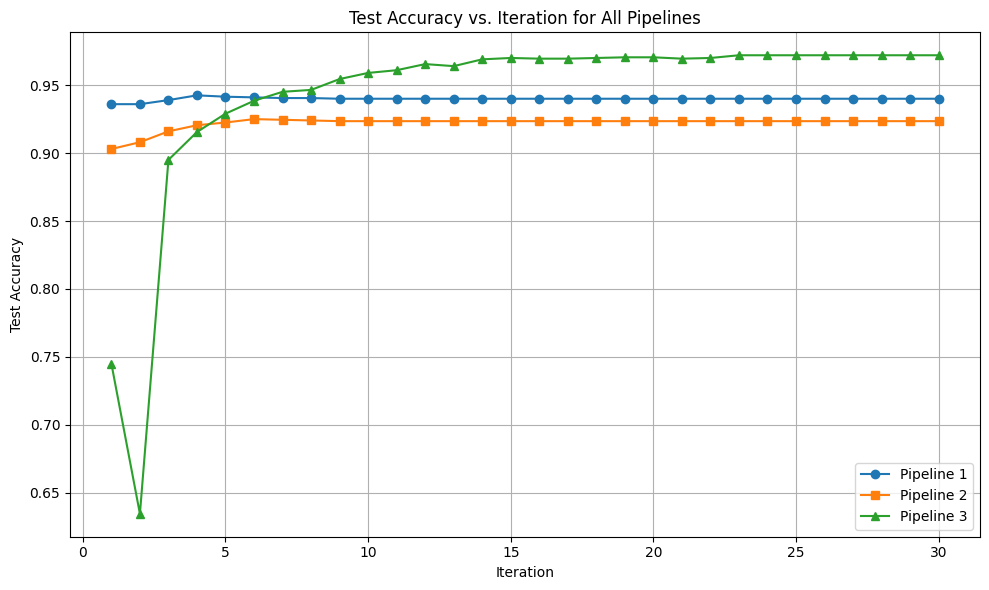
\includegraphics[width=0.8\textwidth]{accs_part3.png}
\caption{Test Accuracy vs. Iteration for All Pipelines. For pipelines that stopped early, the final measured accuracy is held constant to extend the plot to 30 iterations.}
\label{fig:accuracy_vs_iteration}
\end{figure}

\paragraph{Comment:}
Figure~\ref{fig:accuracy_vs_iteration} displays the evolution of test accuracy over 30 iterations for three different pipelines. The graph clearly illustrates the following points:

\begin{itemize}
    \item \textbf{Pipeline 1:}  
    The test accuracy starts at 0.9360 and shows a modest improvement early on, reaching a peak of 0.9425 around iteration 4. Beyond that, the accuracy stabilizes at approximately 0.94. This indicates that while the iterative refinement yields some gains, the performance quickly plateaus.

    \item \textbf{Pipeline 2:}  
    Beginning with a lower accuracy of 0.9030 in iteration 1, Pipeline 2 steadily improves to 0.9235 by iteration 9. The relatively smooth and continuous improvement suggests that the iterative refinement process is effective. However, the overall accuracy remains slightly below that of Pipeline 1.

    \item \textbf{Pipeline 3 (Active Learning):}  
    In contrast, Pipeline 3 starts with a significantly lower accuracy (0.7450) and even dips to 0.6345 in the second iteration. This is likely due to the initial limited seed set and the inherent uncertainty in early pseudo-labeling. Nevertheless, as additional uncertain samples are queried and manually labeled, the accuracy recovers and improves dramatically, reaching 0.9720 by iteration 23. After iteration 23, the accuracy is held constant to extend the curve to 30 iterations. This demonstrates that, despite a slow start, Pipeline 3 eventually surpasses the other pipelines in performance, highlighting the potential benefits of active learning when a sufficient number of iterations are allowed.

    \item \textbf{Overall Comparison:}  
 The graph shows the trade-off between manual labeling time and test accuracy improvement. While Pipeline 1 achieves high and stable accuracy with substantial manual effort, Pipeline 2 shows steady, slightly lower, performance with reduced manual time. Pipeline 3, despite its initially low accuracy, demonstrates the highest eventual test accuracy, making it an attractive approach when maximizing performance is the primary goal.
\end{itemize}


\begin{thebibliography}{9}
\bibitem{geron2019}
Aurélien Géron, \emph{Hands-On Machine Learning with Scikit-Learn, Keras, and TensorFlow}, 2nd Edition, O'Reilly Media, 2019.
\end{thebibliography}



\end{document}

